%! TEX root = ./main.tex

% preamble

\documentclass{article}
% \usepackage{ulem}
\usepackage[fontset=windows]{ctex}
\usepackage{NotesCTeX,lipsum}
\usepackage{svg}
\usepackage{outlines}
\usepackage{braket}
\usepackage{siunitx}
\usepackage{wrapfig}
% \usepackage{tabular}
\newcommand{\im}{\mathrm{i}}%
\newcommand{\XX}{\hat{X}}%
\newcommand{\JJ}{\hat{J}}%
\newcommand{\RR}{{\mathbb{R}}}
\newcommand{\RHat}{\hat{R}}%
\newcommand{\tp}{^{\textup{T}}} %矩阵转置 % 覆盖 physics 宏包的 Trace

% \usepackage[english]{babel}
% https://github.com/gpoore/minted/issues/159
\usepackage[outputdir=latex.out]{minted}
\usemintedstyle{mathematica}
\definecolor{LightGray}{gray}{0.95}

% \code{language}{filename}
% eg: \code{wolfram}{./a.mma}
% eg: \code{python}{./a.py}
\newcommand{\code}[2]{%
\inputminted[%
linenos,
baselinestretch=1.2,
bgcolor=LightGray]{#1}{#2}}
\usepackage[capitalise]{cleveref}
\crefname{equation}{式}{式} 
\crefname{figure}{图}{图} 
\crefname{table}{表}{表} 
\crefname{appendix}{附录}{附录} 
% \crefname{enumi}{条目}{条目} 
\newcommand{\crefpairconjunction}{~和~} 
\newcommand{\crefmiddleconjunction}{、} 
\newcommand{\creflastconjunction}{~和~} 
\newcommand{\crefpairgroupconjunction}{~和~} 
\newcommand{\crefmiddlegroupconjunction}{、} 
\newcommand{\creflastgroupconjunction}{~和~} 
\newcommand{\crefrangeconjunction}{~} 

\DeclareMathOperator{\rref}{rref}
% \renewcommand{\bigO}[1]{$\mathcal{O}(#1)$}
\newcommand{\red}[1]{\textcolor{red}{#1}}
\newcommand{\blue}[1]{\textcolor{blue}{#1}}
% highlight
\newcommand{\hl}[1]{\colorbox{BurntOrange}{#1}}
\newcommand{\matr}[1]{\mathbf{#1}} % undergraduate algebra version
% \newcommand{\matr}[1]{\bm{#1}}     % ISO complying version

% https://tex.stackexchange.com/questions/227639/redefine-emph-to-be-both-bold-and-italic
\let\emph\relax % there's no \RedeclareTextFontCommand
\DeclareTextFontCommand{\emph}{\color{red}\em}

% preamble

\documentclass{article}
% \usepackage{ulem}
\usepackage[fontset=windows]{ctex}
\usepackage{NotesCTeX,lipsum}
\usepackage{svg}
\usepackage{outlines}
\usepackage{braket}
\usepackage{siunitx}
\usepackage{wrapfig}
% \usepackage{tabular}
\newcommand{\im}{\mathrm{i}}%
\newcommand{\XX}{\hat{X}}%
\newcommand{\JJ}{\hat{J}}%
\newcommand{\RR}{{\mathbb{R}}}
\newcommand{\RHat}{\hat{R}}%
\newcommand{\tp}{^{\textup{T}}} %矩阵转置 % 覆盖 physics 宏包的 Trace

% \usepackage[english]{babel}
% https://github.com/gpoore/minted/issues/159
\usepackage[outputdir=latex.out]{minted}
\usemintedstyle{mathematica}
\definecolor{LightGray}{gray}{0.95}

% \code{language}{filename}
% eg: \code{wolfram}{./a.mma}
% eg: \code{python}{./a.py}
\newcommand{\code}[2]{%
\inputminted[%
linenos,
baselinestretch=1.2,
bgcolor=LightGray]{#1}{#2}}
\usepackage[capitalise]{cleveref}
\crefname{equation}{式}{式} 
\crefname{figure}{图}{图} 
\crefname{table}{表}{表} 
\crefname{appendix}{附录}{附录} 
% \crefname{enumi}{条目}{条目} 
\newcommand{\crefpairconjunction}{~和~} 
\newcommand{\crefmiddleconjunction}{、} 
\newcommand{\creflastconjunction}{~和~} 
\newcommand{\crefpairgroupconjunction}{~和~} 
\newcommand{\crefmiddlegroupconjunction}{、} 
\newcommand{\creflastgroupconjunction}{~和~} 
\newcommand{\crefrangeconjunction}{~} 

\DeclareMathOperator{\rref}{rref}
% \renewcommand{\bigO}[1]{$\mathcal{O}(#1)$}
\newcommand{\red}[1]{\textcolor{red}{#1}}
\newcommand{\blue}[1]{\textcolor{blue}{#1}}
% highlight
\newcommand{\hl}[1]{\colorbox{BurntOrange}{#1}}
\newcommand{\matr}[1]{\mathbf{#1}} % undergraduate algebra version
% \newcommand{\matr}[1]{\bm{#1}}     % ISO complying version

% https://tex.stackexchange.com/questions/227639/redefine-emph-to-be-both-bold-and-italic
\let\emph\relax % there's no \RedeclareTextFontCommand
\DeclareTextFontCommand{\emph}{\color{red}\em}

% preamble

\documentclass{article}
% \usepackage{ulem}
\usepackage[fontset=windows]{ctex}
\usepackage{NotesCTeX,lipsum}
\usepackage{svg}
\usepackage{outlines}
\usepackage{braket}
\usepackage{siunitx}
\usepackage{wrapfig}
% \usepackage{tabular}
\newcommand{\im}{\mathrm{i}}%
\newcommand{\XX}{\hat{X}}%
\newcommand{\JJ}{\hat{J}}%
\newcommand{\RR}{{\mathbb{R}}}
\newcommand{\RHat}{\hat{R}}%
\newcommand{\tp}{^{\textup{T}}} %矩阵转置 % 覆盖 physics 宏包的 Trace

% \usepackage[english]{babel}
% https://github.com/gpoore/minted/issues/159
\usepackage[outputdir=latex.out]{minted}
\usemintedstyle{mathematica}
\definecolor{LightGray}{gray}{0.95}

% \code{language}{filename}
% eg: \code{wolfram}{./a.mma}
% eg: \code{python}{./a.py}
\newcommand{\code}[2]{%
\inputminted[%
linenos,
baselinestretch=1.2,
bgcolor=LightGray]{#1}{#2}}
\usepackage[capitalise]{cleveref}
\crefname{equation}{式}{式} 
\crefname{figure}{图}{图} 
\crefname{table}{表}{表} 
\crefname{appendix}{附录}{附录} 
% \crefname{enumi}{条目}{条目} 
\newcommand{\crefpairconjunction}{~和~} 
\newcommand{\crefmiddleconjunction}{、} 
\newcommand{\creflastconjunction}{~和~} 
\newcommand{\crefpairgroupconjunction}{~和~} 
\newcommand{\crefmiddlegroupconjunction}{、} 
\newcommand{\creflastgroupconjunction}{~和~} 
\newcommand{\crefrangeconjunction}{~} 

\DeclareMathOperator{\rref}{rref}
% \renewcommand{\bigO}[1]{$\mathcal{O}(#1)$}
\newcommand{\red}[1]{\textcolor{red}{#1}}
\newcommand{\blue}[1]{\textcolor{blue}{#1}}
% highlight
\newcommand{\hl}[1]{\colorbox{BurntOrange}{#1}}
\newcommand{\matr}[1]{\mathbf{#1}} % undergraduate algebra version
% \newcommand{\matr}[1]{\bm{#1}}     % ISO complying version

% https://tex.stackexchange.com/questions/227639/redefine-emph-to-be-both-bold-and-italic
\let\emph\relax % there's no \RedeclareTextFontCommand
\DeclareTextFontCommand{\emph}{\color{red}\em}

\input{../preamble}
\input{choice_question_env}


%%% vim: set ts=2 sts=2 sw=2 isk+=\: et cc=+1 formatoptions+=mM:

% choice_question_env
\newlength{\xxla}
\newlength{\xxlb}
\newlength{\xxlc}
\newlength{\xxld}
\newlength{\lhalf}
\newlength{\lquarter}
\newlength{\lmax}
\newcommand{\options}[4]{
	\par
	\settowidth{\xxla}{(A)~#1~~~}
	\settowidth{\xxlb}{(B)~#2~~~}
	\settowidth{\xxlc}{(C)~#3~~~}
	\settowidth{\xxld}{(D)~#4~~~}

	\ifthenelse{\lengthtest{\xxla>\xxlb}}{\setlength{\lmax}{\xxla}}{\setlength{\lmax}{\xxlb}}
	\ifthenelse{\lengthtest{\xxlc>\lmax}}{\setlength{\lmax}{\xxlc}}{}
	\ifthenelse{\lengthtest{\xxld>\lmax}}{\setlength{\lmax}{\xxld}}{}
	\setlength{\lhalf}{0.5\linewidth}
	\setlength{\lquarter}{0.25\linewidth}
	\ifthenelse{\lengthtest{\lmax>\lhalf}}
	{
		\begin{enumerate}[label=(\Alph*),parsep=0ex,itemsep=0ex,leftmargin=2em, topsep=0ex]
			\item #1
			\item #2
			\item #3
			\item #4
		\end{enumerate}
	}
	{
		\ifthenelse{\lengthtest{\lmax>\lquarter}}
		{
			\makebox[\lhalf][l]{(A)~#1~~~}%
			\makebox[\lhalf][l]{(B)~#2~~~}%

			\makebox[\lhalf][l]{(C)~#3~~~}%
			\makebox[\lhalf][l]{(D)~#4~~~}%
		}
		{
			\makebox[\lquarter][l]{(A)~#1~~~}%
			\makebox[\lquarter][l]{(B)~#2~~~}%
			\makebox[\lquarter][l]{(C)~#3~~~}%
			\makebox[\lquarter][l]{(D)~#4~~~}%
		}
	}
}




%%% vim: set ts=2 sts=2 sw=2 isk+=\: et cc=+1 formatoptions+=mM:



%%% vim: set ts=2 sts=2 sw=2 isk+=\: et cc=+1 formatoptions+=mM:

% choice_question_env
\newlength{\xxla}
\newlength{\xxlb}
\newlength{\xxlc}
\newlength{\xxld}
\newlength{\lhalf}
\newlength{\lquarter}
\newlength{\lmax}
\newcommand{\options}[4]{
	\par
	\settowidth{\xxla}{(A)~#1~~~}
	\settowidth{\xxlb}{(B)~#2~~~}
	\settowidth{\xxlc}{(C)~#3~~~}
	\settowidth{\xxld}{(D)~#4~~~}

	\ifthenelse{\lengthtest{\xxla>\xxlb}}{\setlength{\lmax}{\xxla}}{\setlength{\lmax}{\xxlb}}
	\ifthenelse{\lengthtest{\xxlc>\lmax}}{\setlength{\lmax}{\xxlc}}{}
	\ifthenelse{\lengthtest{\xxld>\lmax}}{\setlength{\lmax}{\xxld}}{}
	\setlength{\lhalf}{0.5\linewidth}
	\setlength{\lquarter}{0.25\linewidth}
	\ifthenelse{\lengthtest{\lmax>\lhalf}}
	{
		\begin{enumerate}[label=(\Alph*),parsep=0ex,itemsep=0ex,leftmargin=2em, topsep=0ex]
			\item #1
			\item #2
			\item #3
			\item #4
		\end{enumerate}
	}
	{
		\ifthenelse{\lengthtest{\lmax>\lquarter}}
		{
			\makebox[\lhalf][l]{(A)~#1~~~}%
			\makebox[\lhalf][l]{(B)~#2~~~}%

			\makebox[\lhalf][l]{(C)~#3~~~}%
			\makebox[\lhalf][l]{(D)~#4~~~}%
		}
		{
			\makebox[\lquarter][l]{(A)~#1~~~}%
			\makebox[\lquarter][l]{(B)~#2~~~}%
			\makebox[\lquarter][l]{(C)~#3~~~}%
			\makebox[\lquarter][l]{(D)~#4~~~}%
		}
	}
}




%%% vim: set ts=2 sts=2 sw=2 isk+=\: et cc=+1 formatoptions+=mM:



%%% vim: set ts=2 sts=2 sw=2 isk+=\: et cc=+1 formatoptions+=mM:

\title{Demo}
\author{X}

\date{\today}

\begin{document}
% \maketitle
 % \tableofcontents
%! TEX root = debug.tex
% 统计力学
配分函数与热力学量
\begin{equation}
  Z(T,V) = \int e^{-\beta \varepsilon} \dd{\omega} 
  \label{eq:partion_function}
\end{equation}
\begin{equation*}
  U = - N \pdv{\beta} \ln Z
\end{equation*}
\begin{equation*}
  S  = N k T ( \ln Z - \beta \pdv{\beta} \ln Z )
\end{equation*}
\begin{equation}
  F = U -TS = - NkT \ln Z
  \label{eq:FreeEnergy}
\end{equation}
\begin{theorem}[马休定理]
  给出\(F(T,V)\)就能求出一切热力学量。
  \label{th:马休定理}
\end{theorem}
根据定理\ref{th:马休定理}和Eq.~\eqref{eq:FreeEnergy}和Eq.~\eqref{eq:partion_function}得出:给出\(Z(T,V)\)就能求出一切热力学量


%%% vim: set ts=2 sts=2 sw=2 isk+=\: et cc=+1 formatoptions+=mM:

%! TEX root = ./main.tex
% Rayleigh-Jeans

\subsubsection{傅里叶级数}%

\begin{figure}[h]
	\centering
	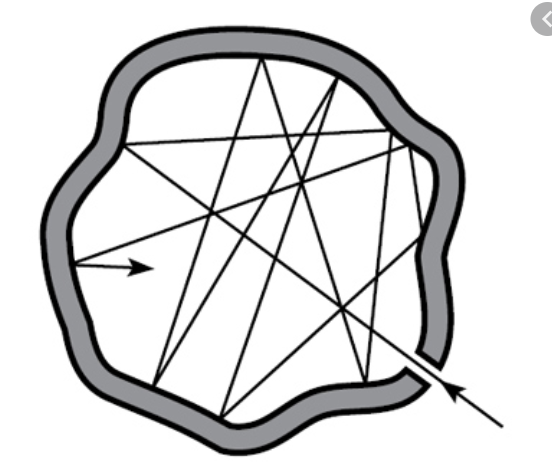
\includegraphics[width=0.2\linewidth]{figures/cavity.png}
	\caption{Cavity}%
	\label{fig:cavity}
\end{figure}

黑体辐射达到平衡后,源给场多少能量,场也给源多少能量。
由源产生的电磁波满足波动方程
\begin{equation}
	\label{eq:wave_eq}
	\laplacian{\psi} - \frac{1}{c^2} \pdv[2]{\psi}{t}=0
\end{equation}

\begin{note}
没有人会去背这个方程,因为这个方程其实就是对闵科夫斯基空间的四个基矢$[x,y,z,ict]$的二阶偏导:
\[
	\left(\pdv[2]{x} +\pdv[2]{y} +\pdv[2]{z} +\pdv[2]{ict} \right)\psi = 0
\]
\end{note}

方程\eqref{eq:wave_eq}的通解就等于特解的线性叠加。

任何一组连续振动的体系都等效于一组谐振子。
任何电磁波都能分解为单色波的叠加。
黑体辐射的能量密度,可以由无数个简谐振子组成。
实际上,这个辐射源就等效于一组谐振子,这些谐振子有不同的频率,就出来不同频率的平面波,把他们叠加,就出来了电磁场。

我们用一个尝试解带入:
\begin{equation}
	\begin{aligned}
		\label{eq:superposition}
			\Psi = \sum_{k} \psi_k  \\
			\psi_k(x,y,z,t)=q_k(t)\exponential(ik\vdot r)
	\end{aligned}
\end{equation}

\begin{align*}
	\sum_{k} \left[ q_k(t) \laplacian \exp(ik\vdot r) - \frac{1}{c^2} \exp(ik \vdot r) \ddot{q_k}(t) \right] = 0 \\
	\laplacian{\exp(i\vb{k}\vdot\vb{r})} = - k^2 \exp(i\vb{k}\vdot\vb{r}) \\ 
	\ddot{q_k}(t)+c^2 k^2 q_k(t) = 0\\
	\omega^k=ck= \frac{2\pi}{\lambda}c=2\pi \nu_k\\
	q_k(t)=A\exp(-i \omega_k t)
\end{align*}

解得

\begin{equation}
	\psi_k(x,y,z,t)=A\exp[ -i(\omega_k t-\vb{k}\vb{r}) ]
\end{equation}


\subsubsection{箱归一化}%

这个解是在没有边界的情况得出的,若有边界应该怎么办呢:
% TODO 加黑体辐射空腔图

假设周期性边界条件:

\begin{subequations}
	\begin{align}
		\psi(x,y,z,t) = \psi(x+L,y,z,t)\\
		\psi(x,y,z,t) = \psi(x,y+L,z,t)\\
		\psi(x,y,z,t) = \psi(x,y,z+L,t)
	\end{align}
\end{subequations}
\begin{subequations}
	\begin{align}
	e^{i k_x L} = 1\\
	e^{i k_y L} = 1\\
	e^{i k_z L} = 1
	\end{align}
\end{subequations}
\begin{subequations}
	\begin{align}
		k_x L = 2\pi n_x \quad k_x=\frac{2\pi}{L}n_x  \quad (n_x=0,\pm 1,\pm 2, \ldots)\\
		k_y L = 2\pi n_y \quad k_y=\frac{2\pi}{L}n_y  \quad (n_y=0,\pm 1,\pm 2, \ldots)\\
		k_z L = 2\pi n_z \quad k_z=\frac{2\pi}{L}n_z  \quad (n_z=0,\pm 1,\pm 2, \ldots)
	\end{align}
\end{subequations}
\begin{equation*}
	\omega_k=2\pi \nu_k = c|\vb{k}| = \frac{2\pi}{L}c\sqrt{n_x^2+n_y^2+n_z^2} 
\end{equation*}
%TODO k 空间到 n 空间的配图

从$n$空间到$k$空间只相差了一个系数,设这个系数为 $\lambda$, 即$\lambda = \left(\frac{L}{2 \pi}\right)^3 = \frac{V}{\left(2 \pi\right)^3}$。现在随便划出一个体积 $\Delta V=\Delta n_x \Delta n_y \Delta n_z$,里面的状态数在数值上就等于n空间的体积:
\begin{equation}
	\begin{aligned}
		\label{eq:space}
		\text{状态数} &=  \Delta n_x \Delta n_y \Delta n_z \\
		&= \lambda \Delta k_x \Delta k_y \Delta k_z \\
		&=   \frac{L}{2 \pi} ^3 \Delta k_x \Delta k_y \Delta k_z  \\
		&=   \frac{V}{{\left( 2 \pi \right)}^3} \Delta k_x \Delta k_y \Delta k_z
	\end{aligned}
\end{equation}

数出在 $\abs{\vectorbold{k}} \sim \abs{\vectorbold{k}} + \dd \abs{\vectorbold{k}}$ 的状态数,只要算出 k 空间球壳的体积,再乘 $\lambda$

笛卡尔坐标转换为球坐标, 并考虑到电磁波的两种独立的偏振,需要乘2

\begin{equation}
	Z_k \dd k = \lambda \cdot \dd k \int_{0 }^{\pi } \sin\theta \dd{\theta}   \int_{0 }^{2\pi } \dd{\phi}  = \lambda \cdot 4 \pi k^2 \cdot \dd k = \frac{V}{(2 \pi)^3} \cdot 4 \pi k^2 \cdot \dd k
\end{equation}

$|\vb{k}| \to \omega $ $(k=\frac{\omega}{c})$
\begin{equation}
	Z'_k d\omega = \frac{4 \pi V}{(2 \pi)^3} \left(\frac{\omega}{c}\right)^2 \dd{\left(\frac{\omega}{c}\right)}  = \frac{4 \pi V}{(2 \pi )^{3}} \frac{\omega^2 d\omega}{c^3}
\end{equation}

\begin{equation*}
	Z_\omega \dd\omega = \frac{V \pi \omega^2 \dd\omega}{(2 \pi c)^3}
\end{equation*}

$ \omega \to \nu $ ($\omega = 2 \pi \nu$)
\begin{equation*}
	Z_\nu \dd \nu = \frac{V}{c^3} 8 \pi \nu^2 \dd \nu
\end{equation*}

设频率在 $\nu \sim \nu + \dd \nu$ 区间的态密度为 $\rho_\nu$
\begin{equation*}
	\rho_\nu = Z_\nu = \frac{V}{c^3} 8 \pi \nu^2 
\end{equation*}

其能量:
\begin{equation}
	\label{eq:Density_of_States}
	\rho_\nu \dd \nu \overline{\varepsilon_\nu}= \frac{8 \pi \nu^2}{c^3} \dd \nu \vdot \overline{\varepsilon_\nu}
\end{equation}

能均分定理。假设:能量是连续的,能量是动量的连续函数,求和变成积分\footnote{要真正解决这个问题,需要普朗克能量量子化,需要能量是频率的函数, 盲猜,什么函数最容易,正比最容易,所以先猜 $E(\nu)=h\nu$,类比傅里叶级数的振幅?这是后话。}:


\begin{equation}
	\label{eq:equipartition_theorem_of_energy}
	\overline{\varepsilon_\nu} = \frac{\overline{p^2} }{2m} + \overline{\frac{1}{2}m\omega^2q^2} = kT
\end{equation}

把方程\eqref{eq:equipartition_theorem_of_energy}带入方程\eqref{eq:Density_of_States}  得

\begin{equation}
	\rho_\nu \dd\nu = \frac{8 \pi \nu^2}{c^3} kT \dd \nu
\end{equation}


\section{极限}%
\begin{exercise}
	\begin{equation*}
		\lim_{\substack{x \to 0 \\ y \to 0}} \frac{xy}{\sqrt{x^2 + y^2}} = 0
	\end{equation*}
\end{exercise}
\begin{proof}
	\begin{equation}
		\left|  \frac{xy}{\sqrt{x^2 + y^2}} \right|
		\leq
		\frac{(x^2+y^2) / 2}{ \sqrt{x^2 + y^2} }
		=
		\frac{\sqrt{x^2 + y^2}}{2}
	\end{equation}
	\mn{
		\(
		\left|xy\right| \leq (x^2 + y^2)/2
		\)
	}
	即:
	\begin{equation*}
		0
		\leq
		\left|  \frac{xy}{\sqrt{x^2 + y^2}} \right|
		\leq
		\frac{\sqrt{x^2 + y^2}}{2}
	\end{equation*}
	\marginnote{
		\( \begin{aligned}
			 & \forall \varepsilon > 0                                                          \\
			 & \exists \delta = 2\varepsilon \qc 0 < \rho <\delta                               \\
			 & \st \frac{\sqrt{x^2 + y^2}}{2} = \frac{\rho}{2} < \frac{\delta}{2} = \varepsilon
		\end{aligned} \)
	}
	\begin{equation}
		0
		\leq
		\lim_{\substack{x \to 0 \\ y \to 0}}
		\left|  \frac{xy}{\sqrt{x^2 + y^2}} \right|
		\leq
		\lim_{\substack{x \to 0 \\ y \to 0}}
		\frac{\sqrt{x^2 + y^2}}{2}
		=
		0
	\end{equation}

	\( 		\therefore \)
	\begin{equation}
		\lim_{\substack{x \to 0 \\ y \to 0}} \frac{xy}{\sqrt{x^2 + y^2}} = 0
	\end{equation}
\end{proof}
\begin{exercise}
	设
	\begin{equation*}
		f(x) =
		\begin{cases}
			\frac{(x+y) \sin xy }{x^2 + y^2} \qc x^2 + y^2 \neq 0 \\
			0 \qc x^2 + y^2 = 0
		\end{cases}
	\end{equation*}
	证明:
	\( f(x,y) \) 在 \( (0,0) \) 连续但不可微
\end{exercise}
\begin{proof}
	由于
	\begin{equation*}
		\left| \frac{(x+y) \sin xy }{x^2 + y^2}  \right|
		\leq
		\left| \frac{(x+y) xy}{2 x y}  \right|
		\leq
		\frac{\left| x + y \right|}{2}
		\leq
		\frac{\left| x \right|}{2}
		+
		\frac{\left| y \right|}{2}
	\end{equation*}
	\( \forall \varepsilon > 0 , \exists \delta =  \varepsilon \)  当 \( \left| x \right| \bra{ \delta , \left| y \right| < \delta } \) 时
	\begin{equation*}
		\left| f(x,y) - f(0,0) \right|
		=
		\left| \frac{(x+y) \sin xy }{x^2 + y^2}  \right|
		<
		\frac{\left| x \right|}{2}
		+
		\frac{\left| y \right|}{2}
		<
		\varepsilon
	\end{equation*}
	即:
	\begin{equation}
		\lim_{\substack{ x \to 0 \\ y \to 0 } } f(x,y)
		=
		f(0,0)
		=0
	\end{equation}
	故, \( f(x,y) \) 在点 \( (0,0) \) 处连续, 下证 \( f(x,y) \)在点\(  \)
	\begin{align*}
		f_x'(0,0) & = \lim_{x \to 0} \frac{ f(x,0) - f(0,0) }{ x - 0 } \\
		          & = \frac{ \frac{x \vdot 0}{x^2} }{x}                \\
		          & = \frac{0}{x^3} = 0
	\end{align*}
	同理 \( f'_y(0,0) = 0 \)
	令
	\begin{equation*}
		\Delta \omega = f(x,y) - f(0,0) - f'_x(0,0) \Delta x - f'_y(0,0) \Delta y =  \frac{(x+y) \sin xy }{x^2 + y^2}
	\end{equation*}
	而\marginnote{
		\begin{equation*}
			\begin{aligned}
				 & \lim_{\substack{ \rho \to 0           \\ y = kx }}
				\frac{ k+1 }{(k^2 +1)^{\frac{3}{2}}}
				\cdot
				\frac{ \sin k x^2 }{x^2}                 \\
				 & =
				\lim_{\substack{ \rho \to 0              \\ y = kx }}
				\frac{ k+1 }{(k^2 +1)^{\frac{3}{2}}}
				\lim_{\substack{ \rho \to 0              \\ y = kx }}
				\frac{ k \sin \red{k x^2} }{\red{k x^2}} \\
				 & =
				\frac{(k+1)k}{ (k^2 + 1)^{\frac{3}{2}} } \quad \text{与\( k \)有关}
			\end{aligned}
		\end{equation*}
	}
	\begin{equation*}
		\begin{aligned}
			\lim_{ \rho \to 0 }
			\frac{\Delta \omega}{\rho}
			 & =
			\lim_{ \rho \to 0 }
			\frac{(x+y) \sin xy }{(x^2 + y^2)^{\frac{3}{2}}} \\
			 & =
			\lim_{\substack{ \rho \to 0                      \\ y = kx }}
			\frac{(x+y) \sin xy }{(x^2 + y^2)^{\frac{3}{2}}} \\
			 & =
			\lim_{\substack{ \rho \to 0                      \\ y = kx }}
			\frac{ k+1 }{(k^2 +1)^{\frac{3}{2}}}
			\cdot
			\frac{ \sin k x^2 }{x^2}                         \\
			 & =
			\frac{(k+1)k}{ (k^2 + 1)^{\frac{3}{2}} } \quad \text{与\( k \)有关}
		\end{aligned}
	\end{equation*}
\end{proof}

\begin{exercise}
	将 \( f(x) = \arctan \frac{1+x}{1-x} \)展成\( x \)的幂级数。
	\begin{margintable}
		\begin{tabularx}{\marginparwidth}{|X}
			Section~. Motivation        \\
			Section~. Required Packages \\
			Section~. Margins           \\
		\end{tabularx}
	\end{margintable}
	解:
	\begin{align*}
		 & f'(x) = \frac{1}{1 + (\frac{1+x}{1-x})^2} \vdot \frac{1 - x - (1+x) (-1)}{ (1-x)^2 }                        \\
		 & = \frac{2}{2+2x^2} = \frac{1}{1+x^2} = \sum_{n=0}^{\infty)} (-1)^n x^{2n} \quad \text{收敛半径}(-1 < x < 1)
	\end{align*}
	\marginnote{
		令
		\( x = -1 \)
		\begin{gather*}
			0 = \frac{\pi}{4} + \sum_{n=0}^\infty (-1)^{n+1} \frac{1}{2n+1} \\
			-\sum_{n=0}^\infty (-1)^{n+1} \frac{1}{2n+1}
			=
			\frac{\pi}{4} \\
			4 \sum_{n=0}^\infty (-1)^{n+2} \frac{1}{2n+1}
			=
			\pi \\
			4 \sum_{n=0}^\infty (-1)^{n} \frac{1}{2n+1}
			=
			\pi
		\end{gather*}
		令 \( n=m-1 \)
		\begin{equation*}
			\begin{aligned}
				\pi
				 & =
				4 \sum_{m=1}^\infty (-1)^{m-1} \frac{1}{2m-1} \\
				 & =
				4 \sum_{n=1}^\infty (-1)^{n-1} \frac{1}{2n-1}
			\end{aligned}
		\end{equation*}
		误差(莱布尼兹判别法)
		\begin{equation*}
			\left| R_n \right| \leq \frac{4}{\underbrace{2n+1}_{u_{n+1}}}
		\end{equation*}
	}
	\begin{gather*}
		\int_0^x f'(x) \dd x = \sum_{n=0}^\infty (-1)^n \int_0^x x^{2n} \dd x  \\
		f(x) - f(0) =
		\sum_{n=0}^\infty (-1)^n \frac{x^{2n+1}}{2n+1}\\
		f(x) - f(0) = \sum_{n=0}^\infty (-1)^n \frac{x^{2n+1}}{2n+1}\\
		f(0) = \arctan 1 = \frac{\pi}{4}\\
		\therefore f(x) = \arctan \frac{1+x}{1-x} = \frac{\pi}{4} +
		\sum_{n=0}^\infty (-1)^n \frac{x^{2n+1}}{2n+1}
	\end{gather*}
\end{exercise}


\section{热扩散方程}%
如图~\ref{fig:热流与温度的关系} 可知
\begin{marginfigure}
	\includesvg[width=0.8\textwidth]{figures/热流与温度的关系.svg}
	\caption{热流与温度的关系。不管人为选定的\( x \)轴的方向如何,热量总是自发地从高温热源流向低温热源。}
	\label{fig:热流与温度的关系}
\end{marginfigure}
若\( T_2 - T_1 >0 \)那么热量从红线向蓝线流动\( \vb{h} \)的方向向左

设\( \Delta J \)
为从1到2传递的热量的大小,显然由于\( T_2>T_1 \),热量应该由2传到1,所以\( \Delta J \)为负值。

直觉上,\( \Delta J \)
\begin{itemize}
	\item 与厚度\( \Delta s  \)成负相关
	\item 与温差 \( \Delta T \)成正相关
	\item 与面积 \( \Delta A \)成正相关
	\item 与材料的性质,即热导率 \( \kappa \)有关
\end{itemize}
我们简单粗暴地写成反比和正比的形式(对于大多数金属材料确实近似如此)
\begin{equation*}
	\Delta J = \red{-} \kappa \Delta A  \Delta T / \Delta s
\end{equation*}
\sn{\red{这里的负号体现着热二定律}}
设 \( h = \frac{\Delta J}{\Delta A} \)为单位面积的传递的热量,称为热流
\begin{equation*}
	h = - \kappa \Delta T / \Delta s
\end{equation*}
\begin{equation*}
	h = - \kappa \frac{\dd T}{\dd s} \qq{或} h_x = - \kappa \dv{T}{x}
\end{equation*}
对于三维情况:
\begin{align*}
	h_x = - \kappa \pdv{T}{x} \\
	h_y = - \kappa \pdv{T}{y} \\
	h_z = - \kappa \pdv{T}{z}
\end{align*}
\begin{equation}
	\vb{h} = - \kappa \grad T
	\label{eq:热流}
\end{equation}

选取一小块体积 \( \Delta V \), 设 \( \Delta V \) 中含有热量 \( \Delta Q \), \( \Delta Q \) 的减少率等于流出去的热量(热流\( \vb{h} \)对该表面的环积分)
\begin{equation}
	-	\pdv{\Delta Q}{t} = \iint_{\partial (\Delta V)} \vb{h} \vdot \vb{n} \dd A = \div \vb{h} \Delta V
\end{equation}
\begin{equation*}
	-\pdv{t}(\frac{\Delta Q}{\Delta V}) = \div \vb{h}
\end{equation*}
设\( q = \frac{\Delta Q}{\Delta V} \) 为单位体积内含有的的热量
\begin{equation}
	-\pdv{q}{t} = \div \vb{h}
	\label{eq:热量连续性}
\end{equation}
\begin{equation}
	q = c_v T
	\label{eq:热容}
\end{equation}
把式~\eqref{eq:热流}和式~\eqref{eq:热容} 带入式~\eqref{eq:热量连续性}
\begin{equation}
	\pdv{T}{t} = \frac{\kappa}{c_v} \laplacian T
	\label{eq:热扩散方程}
\end{equation}
式~\eqref{eq:热扩散方程} 常被写为:
\begin{equation}
	\pdv{T}{t} =  D \laplacian T
\end{equation}
\( D \)称为扩散常数,这里等于\( \frac{\kappa}{c_v} \)。

\begin{itemize}
	\item Lagrangian 代表着全部的物理
	      \begin{itemize}
		      \item 物理系统本身
		            \begin{enumerate}
			            \item 物理系统本身
			            \item 物理规律对系统的支配
		            \end{enumerate}
		      \item 物理规律对系统的支配
	      \end{itemize}
	\item 三个守恒来自同一个原理:\( \var L = 0 \)
\end{itemize}


Giving a Temperature field, say \( T \), we can write down the full version of \( \dd T \)
\begin{equation}
	\begin{aligned}
		\dd T
		 & =
		\pdv{T}{x} \dd x +
		\pdv{T}{y} \dd y +
		\pdv{T}{z} \dd z                         \\
		 & =
		\mqty[
		\pdv{T}{x}                               \\
		\pdv{T}{y}                               \\
			\pdv{T}{z}
		]
		\vdot
		\mqty[\dd x                              \\ \dd  y \\ \dd z]
		\\
		 & =
		\mqty[
		\pdv{x}                                  \\
		\pdv{y}                                  \\
			\pdv{z}
		] T
		\vdot
		\dd
		\mqty[x                                  \\ y \\ z]
		 & \mn{不会因为坐标系的改变而改变}=
		\grad T \vdot
		\dd
		\mqty[x                                  \\ y \\ z] \\
		 & =
		\mqty[
		\pdv{x'}                                 \\
		\pdv{y'}                                 \\
			\pdv{z'}
		] T
		\vdot
		\dd
		\mqty[x'                                 \\ y' \\ z']
		 & =
		\grad' T \vdot
		\dd
		\mqty[x'                                 \\ y' \\ z'] \\
		 & = \grad T\vdot  \dd \vb{r}
		= \grad' T \vdot \dd \vb{r}'             \\
		 & = \grad' T \vdot \dd \matr{A} \vb{r}
		= \grad' T \vdot \matr{A} \dd  \vb{r}    \\
		 & = \grad' \matr{A}  T \vdot \dd \vb{r}
		= \grad T \vdot \dd \vb{r}
	\end{aligned}
\end{equation}
\sn{\(\matr{A}\)是旋转矩阵\( \st \vb{r}' = \matr{A} \matr{r} \)}
ie.
\begin{equation}
	\grad = \grad' \matr{A} \qif  \vb{r}' = \matr{A} \matr{r}
\end{equation}
\begin{definition}
	\begin{equation*}
		\grad :=
		\mqty[
			\pdv{x}       \\
			\pdv{y}       \\
			\pdv{z}
		]
	\end{equation*}
	\begin{equation*}
		\vb{r} :=
		\mqty[x          \\ y \\ z]
	\end{equation*}
\end{definition}
% TODO 用一个 ctrl + 字母表示 item
\begin{equation*}
	\dd T
	=
	\grad T \vdot \dd \vb{r}
	=
	\abs{\grad T}  \cos \theta \abs{\dd \vb{r} }
\end{equation*}
\( \theta \) 取 \ang{0} 的时候\( \dd T \)取最大,也就是说 \( \grad T \)的方向是 \( T \)变化最快的方向。

\begin{marginfigure}
	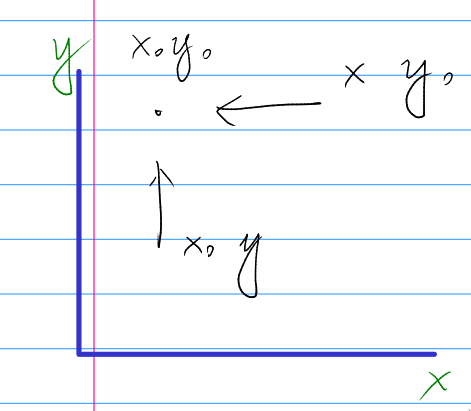
\includegraphics[width=0.8\textwidth]{figures/2021-09-09T203722+0800.png}
\end{marginfigure}
\begin{proof}
	C-R 关系 Cauchy-Riemann equation

	若
	\[
		f'(z) = \lim_{z \to z_0} \frac{ f(z) - f(z_0) }{ z -z_0 } \text{存在} \qc z = x + \im y
	\]
	不论从哪个方向趋于 \( (x_0,y_0) \) 所得都应该是 \( f'(z) \):
	\mn{在欧几里得空间,微小范围,只要从“横平竖直” 两个方向趋近,那么应该是等价的,这里只证明\hl{导数存在 \( \implies \) C-R 关系}}
	\begin{enumerate}
		\item \( (x, y_0) \to (x_0,y_0) \):
		      \begin{align*}
			      f'(z) & = \lim_{z \to z_0} \frac{ f(z) - f(z_0) }{ z -z_0 }                                  \\
			            & =	\lim \frac{  u(x,y_0) + \im  v(x,y_0) - ( u(x_0,y_0) + \im  (v(x_0,y_0)) ) }{x - x_0} \\
			            & = \pdv{u}{x} +  \pdv{\im  v}{x}                                                       \\
			            & = \blue{\pdv{u}{x}} +  \red{\im \pdv{  v}{x}}
		      \end{align*}
		\item \( (x_0, y) \to (x_0,y_0) \):
		      \begin{align*}
			      f'(z) & = \lim_{z \to z_0} \frac{ f(z) - f(z_0) }{ z -z_0 }                                       \\
			            & =	\lim \frac{  u(x_0,y) + \im  v(x_0,y) - ( u(x_0,y_0) + \im  (v(x_0,y_0)) ) }{\im (y - y_0)} \\
			            & = \pdv{u}{\im y} + \pdv{\im v}{\im y}                                                        \\
			            & = \red{- \im  \pdv{u}{y}} + \blue{\pdv{v}{y}}
		      \end{align*}
	\end{enumerate}
	对应项相等有:
	\begin{equation}
		\text{C-R 关系:} \left\{
		\begin{aligned}
			\pdv{u}{x} & = \pdv{v}{y}  \\
			\pdv{u}{y} & = -\pdv{v}{x}
		\end{aligned} \right\}
	\end{equation}
\end{proof}

\begin{equation}
	\oint f(z) \dd{z} = \oint (u+iv)(dx + idy)
\end{equation}
According to Stokes equation:
\begin{equation}
\begin{aligned}
\oint (u+iv)(dx + idy)
&= \oint (udx - vdy) + \im \oint (udy + vdx) \\
&= \int ( \pdv{(-v)}{x} - \pdv{u}{y}  ) \dd{\tau} + \im \int ( \pdv{u}{x} - \pdv{v}{y} ) \dd{\tau} \\
&= 0 + 0 \im
\end{aligned}
\end{equation}

\subsection{平面方程的点法式}%
% \begin{marginfigure}
% 	\begin{center}
% 		\begin{tikzpicture}
% 			\draw[black,thick] (-1,-1) -- (-.06,-.06);
% 			\draw[black,thick] (.06,.06) -- (1,1);
% 			\draw[black,thick] (-1,1) -- (1,-1);
% 			\filldraw[black] (-1,-1) circle (2pt) node[anchor=north] {2};
% 			\filldraw[black] (-1,1) circle (2pt) node[anchor=south] {1};
% 			\filldraw[black] (1,-1) circle (2pt) node[anchor=north] {3};
% 			\filldraw[black] (1,1) circle (2pt) node[anchor=south] {4};
% 		\end{tikzpicture}
% 	\end{center}
% 	\caption{Marginfigure: Tikz}
% \end{marginfigure}
\begin{wrapfigure}{r}{0.30\textwidth}
	\includesvg[width=0.28\textwidth]{figures/平面方程的点法式.svg}
	% \caption{平面方程的点法式}
	% \label{fig:平面方程的点法式}
\end{wrapfigure}
\sn{法向量加一点,确定一个平面}
\begin{marginfigure}
	\begin{flushright}
		\includesvg[width=0.8\textwidth]{figures/平面方程的点法式.svg}
		\caption{平面方程的点法式}
		\label{fig:平面方程的点法式}
	\end{flushright}
\end{marginfigure}
如图~\ref{fig:平面方程的点法式} 所示
\begin{gather*}
	\vb{n} = (A,B,C) \\
	O = (x_0, y_0, z_0)  \\
	P(x,y,z) \\
	\overrightarrow{DP} \perp \vb{n} \\
	(A,B,C) \perp (x-x_0, y-y_0, z-z_0) \\
	A(x-x_0) + B(y-y_0) + C(z-z_0) = 0
\end{gather*}

\begin{equation}
	\label{eq:平面方程的点法式}
	Ax + By + Cz + \underbrace{(- Ax_0 -B y_0 - C z_0 )}_{\text{设为}D} = 0
\end{equation}
\subsection{平面方程的一般式}%
由式~\eqref{eq:平面方程的点法式} 知 平面方程一般式
\begin{equation}
	\label{eq:平面方程一般式}
	Ax + By + Cz + D = 0
\end{equation}
\begin{remark}
	三点确定一个平面。三个点能列出三个方程,故\( A,B,C,D \)中只需要确定三个量就能确定一个平面。\\[2\baselineskip]

	{\itshape 理由:
	\begin{enumerate}
		\item 齐次方程: 只需要算出 \( A,B,C,D \)比例,可以约去
		\item 平面只需要不在同一直线上的三点即可确定
	\end{enumerate}}
\end{remark}
\begin{marginfigure}
	\centering
	\includesvg[width=0.8\textwidth]{figures/condition-of-use.svg}
	\caption{Condition of use}
	\label{fig:condition-of-use}
\end{marginfigure}
Condition of use:
\begin{enumerate}
	\item  The equation can be writen as
	      \( Ax + By + Cz = 0 \),
	      in case the plane \( \Pi \) goes through the origin.
	\item  The equation can be written as \( A x + B y + D =0 \),
	      in case the plane \( \Pi \parallel  Oz \implies C =0 \) (ie. the coefficient of z is 0, C is \( z \) component of the normal vector of \( \Pi \)),
	      as shown as the 1st figure of Fig.~\ref{fig:condition-of-use}
	\item The equation can be written as \( A x + B y =0 \),
	      in case the plane \( \Pi \) goes through the axis \( Oz \)
	      \( \implies
	      \begin{cases}
		      D = 0 \qc \text{goes through the origin} \\
		      C = 0
	      \end{cases}
	      \)
	      , as shown as the 2nd figure of Fig.~\ref{fig:condition-of-use}
\end{enumerate}

\subsection{平面方程的截距式}%
\begin{definition}[平面方程的截距式]
	若平面方程为
	\begin{equation*}
		\frac{x}{a} + \frac{y}{b} + \frac{z}{c} = 1 \quad (a,b,c \neq 0)
	\end{equation*}
	称为截距式。
\end{definition}

该平面经过
\begin{align*}
	(a,0,0) \\
	(0,b,0) \\
	(0,0,c)
\end{align*}
\( a,b,c \)分别为在
\( x \)轴,
\( y \)轴,
\( z \)轴上的截距(不一定为正)

\begin{equation*}
	A x + By +Cz + D =0 \implies
	\frac{x}{- \frac{D}{A}} + \frac{y}{- \frac{D}{B}} + \frac{z}{- \frac{D}{C}} = 1
	\ \ (A,B,C,D \neq 0)
\end{equation*}

\subsection{平面方程三点式}%
若平面 \( \Pi \)经过不在同一直线上的三点,
\(
M_1(x_1,y_1,z_1),
M_2(x_2,y_2,z_2),
M_3(x_3,y_3,z_3),
\)
或
\(
\mqty[
	x_1&y_1&z_1 \\
	x_2&y_2&z_2 \\
	x_3&y_3&z_3
]
\)
线性无关,求平面 \( \Pi \)的方程。

解法一:
\begin{equation}
	\mqty[
		x_1 & y_1 & z_1 & -1 \\
		x_2 & y_2 & z_2 & -1 \\
		x_3 & y_3 & z_3 & -1
	]
	\mqty[
		A \\ B \\ C \\ D
	]
	=0
\end{equation}

% 	\centering
% 	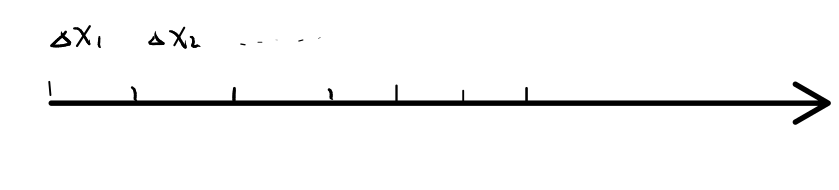
\includegraphics[width=0.8\linewidth]{figures/2021-09-05T122541+0800.png}
% 	\caption{等距分布}%
% \end{figure}
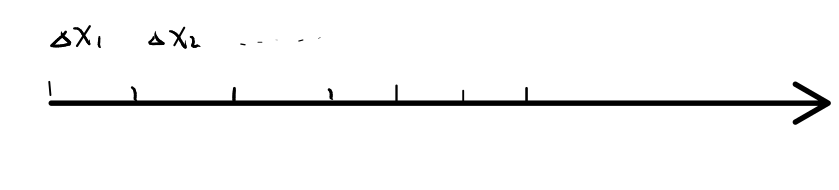
\includegraphics[width=0.8\linewidth]{figures/2021-09-05T122541+0800.png}
\begin{itemize}
	\item 用 \( i \)还是 \( j \)其实无所谓,\( i \) 从 \( 0 \) 取到 \( n \),\( n \) 的大小也无所谓
	\item \( \Delta x_i \)的大小无所谓,只需要 最大的那段\( \max(\{ \Delta x_i, i \in [1, n] \}) \to 0 \)
	\item 所需要表示的只是对应的\emph{加权}的和的极限
	      \begin{enumerate}
		      \item 对应相乘 \(\Delta \psi_i = f_i \vdot \Delta x_i \)
		      \item 求和 \( \sum_i \Delta \psi_i \)
		      \item 取极限 \( \lim_{\max(\{ \Delta x_i \}) \to 0} \sum_i \Delta \psi_i \)
	      \end{enumerate}
\end{itemize}
所以简化书写把\( i \)去掉
\begin{enumerate}
	\item 每一项写成 \( \dd \psi = f \dd x \)
	\item 求和写成 \( \int \dd \psi \)
\end{enumerate}

% MeanValueTheorem


\section{Mean Value Theorem}%
% 中值定理
Fermat Lemma
\( \implies \)
Rolle Theorem
\( \implies \)
Lagrange's Mean Value Theorem
\( \implies \)
Cauchy Mean Value Theorem

\subsection{Fermat Lemma}%
\label{sub:Fermat_Lemma}

\begin{equation*}
\frac{f(x + \Delta x) - f(x)}{\Delta x}
\end{equation*}

\begin{enumerate}
	\item Minimum: 
	\begin{enumerate}
		\item If \( \Delta x > 0 \), \( f(x + \Delta x) - f(x) > 0\) , 
\( \frac{f(x + \Delta x) - f(x)}{\Delta x} >0 \)
		\item If \( \Delta x < 0 \), \( f(x + \Delta x) - f(x) < 0\) 
\( \frac{f(x + \Delta x) - f(x)}{\Delta x} <0 \)
	\end{enumerate}
	\item Maximum 
\begin{enumerate}
		\item If \( \Delta x > 0 \), \( f(x + \Delta x) - f(x) < 0\) , 
\( \frac{f(x + \Delta x) - f(x)}{\Delta x} <0 \)
		\item If \( \Delta x < 0 \), \( f(x + \Delta x) - f(x) > 0\) 
\( \frac{f(x + \Delta x) - f(x)}{\Delta x} >0 \)
	\end{enumerate}
\end{enumerate}
\begin{equation*}
	h(\xi) = \frac{f(x + \xi) - f(x)}{\xi}
\end{equation*}
Zero point theorem:
\begin{enumerate}
	\item If \( h(\xi^-) < 0 \) and \( h(\xi^+) > 0 \), then \( h(\xi) = 0 \)
	\item If \( h(\xi^-) > 0 \) and \( h(\xi^+) < 0 \), then \( h(\xi) = 0 \)
\end{enumerate}

\subsection{Rolle Theorem}%
\label{sub:Rolle_Theorem}

Give an arbitrary curve. Two possibilities:
\begin{enumerate}
	\item Extremum is one of the endpoints of the curve. The curve is a straight line. \( \forall \xi \in (x_1, x_2), f'(\xi) = 0 \).
	\item Extremum in the middle of the curve. There must be a point, say \( \xi \), \( s.t. f'(\xi) = 0 \), according to \cref{sub:Fermat_Lemma}.
\end{enumerate}

So if 
\begin{enumerate}
	\item continuous in \( [x_1, x_2] \) 
	\item differentiable in \( (x_1, x_2) \) 
	\item \( f(x_1) = 0, f(x_2) = 0 \),
\end{enumerate}
\( \exists \xi \in (x_1, x_2) s.t. f'(\xi) = 0 \).
\subsection{Lagrange's Mean Value Theorem}%
\sidenote{
\begin{equation*}
	\Delta y = y'(\xi) \Delta x \qc \xi \in (x, x + \Delta x)
\end{equation*}
If \( \Delta x \to 0 \), then \( \xi \to x \)
\begin{align*}
	\Delta y &= y'(\xi) \\ 
					 &\approx  y'(x) \Delta x \qc \xi \in (x, x + \Delta x)
\end{align*}
\( \dd x = \Delta x, \Delta x \to 0 \)
\begin{equation*}
	\dd y = y'(x) \dd x 
\end{equation*}
% which is fundamental theorem of Calculus.
}
Rotate the x y coordinate system according to Section~\ref{sub:Rolle_Theorem}.
\begin{equation}
	\frac{y_2 - y_1}{x_2 - x_1} = y'(\xi) \qc \xi \in (x_1, x_2) %TODO []  or ()
	\label{eq:LagrangeTheorem}
\end{equation}


\subsection{Cauchy Mean Value Theorem}%
	According to Eq.~\eqref{eq:LagrangeTheorem} 
\begin{equation*}
\begin{aligned}
	\frac{f_2 - f_1}{g_2 - g_1} = f'(\xi) &= \eval{\dv{f}{g}}_{t = \xi} \\ %TODO []  or () 
	&= \eval{\left(\dv{f}{t} \vdot
	\dv{t}{g}\right)}_{t = \xi} 
	= \frac{f'(\xi)}{g'(\xi)}
	\qc \xi \in (t_1,t_2)
\end{aligned}
\end{equation*}
i.e.
\begin{equation}
	\frac{f(t_2) - f(t_1)}{g(t_2) - g(t_1)} = 
	= \frac{f'(\xi)}{g'(\xi)}
	\qc \xi \in (t_1,t_2)
\end{equation}

%%% vim: set ts=2 sts=2 sw=2 isk+=\: et cc=+1 formatoptions+=mM:

% !TEX root = main.tex
% 电势和电场

\section{ \( \vb{E} = - \grad \varphi \) }%

在标量场\( \varphi \)中(\( \varphi \)是电势),将一单位电荷从 1 移到 2,整个过程是准静态的。假设从1到2的电势升高 \( \Delta \varphi \)。\sn{就算是降低也没有关系,那么 \( \Delta \varphi \)是负的就行了}
\begin{equation*}
	\Delta \varphi = \varphi(x_2) - \varphi(x_1) 
	= 
	\pdv{\varphi}{x} \Delta x
\end{equation*}
那么外力(非静电力)需要对此单位电荷做功\( \Delta W \) 使之电势升高
\begin{equation*}
	\Delta W = \Delta \varphi
\end{equation*}

在矢量场\( \vb{E} \)中(\( \vb{E} \)是电场强度),由于准静态过程,外力\( \vb{F} \)和静电力\( \vb{E} \)受力平衡:
\begin{equation*}
	\vb{F} + \vb{E}q = 0
\end{equation*}
在数值上
\begin{equation*}
	\vb{F} + \vb{E} = 0
\end{equation*}
由功的定义:
\begin{equation*}
	\Delta W = F \Delta x = -E_x \Delta x
\end{equation*}
可得
\begin{equation*}
	\pdv{\varphi}{x} = - E_x
\end{equation*}
三维情况
\begin{align*}
	\pdv{\varphi}{x} = - E_x \\
	\pdv{\varphi}{y} = - E_y \\
	\pdv{\varphi}{z} = - E_z
\end{align*}
\begin{equation}
	\grad \varphi = -\vb{E}
\end{equation}
综上,从点1到点2,外力做功,在标量场中只要计算一个减法
\begin{equation*}
 \frac{\Delta W}{q}	 = \varphi(\vb{r}_2) - \varphi(\vb{r}_1)
\end{equation*}
而在矢量场中需要计算三个积分
\begin{equation*}
	\frac{\Delta W}{q}	 =\int_{\vb{r}_1}^{\vb{r}_2} - \vb{E} \dd \vb{r}
\end{equation*}

\begin{proof}
	\begin{equation}
		\curl [ f(r) \vu{r} ]
		\label{eq:球对称的力}
	\end{equation}
\end{proof}
\begin{enumerate}
	\item 由库伦定律,点电荷\( q_i \)的电场\( \vb{E}_i \)满足式~\eqref{eq:球对称的力} 
	\item \( \curl \vb{E}_i = 0 \)
	\item 叠加\sn{叠加与坐标轴的选取无关}原理 
		\( \curl \left(\sum_i \vb{E}_i\right) = 0 \)
	\item \( \forall \vb{E}, \curl \vb{E} = 0 \). 
	\item 由\( \curl \grad \varphi \equiv 0 \)知,\( \varphi \)必然存在。
\end{enumerate}




%%% vim: set ts=2 sts=2 sw=2 isk+=\: et cc=+1 formatoptions+=mM:

% !TEX root = main.tex
% 伯努力定律

\section{伯努力定律}%

质量守恒,在\( \Delta t \)内,流进来的水的质量和流出去的水的质量相等:
\begin{equation*}
	\Delta m_1 = \Delta m_2
\end{equation*}

能量守恒,在\( \Delta t \)内,流进来的能量和流出去的能量相等:
\begin{equation*}
	\frac{1}{2}
	\Delta m_1 v_1^2 + \Delta m_1 g h_1 + P_1 \Delta V_1
	=
	\frac{1}{2}
	\Delta m_2 v_2^2 + \Delta m_2 g h_2 + P_2 \Delta V_2
\end{equation*}

设水的密度处处一致
\begin{equation*}
	\rho = 
	\frac{\Delta m_1}{\Delta V_1}
	=
	\frac{\Delta m_2}{\Delta V_2}
\end{equation*}


则:

\begin{equation*}
	\frac{1}{2} \rho v^2 + \rho g h + P = \text{Const}
\end{equation*}




%%% vim: set ts=2 sts=2 sw=2 isk+=\: et cc=+1 formatoptions+=mM:
%
% !TEX root = main.tex
% NullSpace

\section{ Null Space }%
Null space contains all special solutions. How many special solutions?
One for every free variable.


Augmented matrix


有解的条件: the condition for solvability

So I can \textbf{proceed} to so

Solvability condition on b
\( Ax = b \) is solvable when \( b \) is in \( C(A) \)
\( b \) has to be a combination of the columns
If a comb of rows of A gives zero \textbf{row}, the same comb of rows of b gives zero.

They are both equivalent to the solvability of the system

To find complete solution to \( Ax = b \)
\begin{enumerate}
	\item \( x_\text{particular} \): Set the free variables to zero. It's ``free''.
\end{enumerate}


\begin{listing}
	\begin{minted}[linenos,numbersep=5pt,frame=lines,framesep=2mm]{matlab}
A = [ 1 2 2 2 1; 0 0 2 4 3 ];
b = [1;3];
AA = [A b; zeros(1,length(A)+1)]
length(AA)
R=rref(AA);
\end{minted}
	\caption{matlab code}
	\label{lst:matlab_code}
\end{listing}

What's free variable?
\( \implies a \to b \)
Reduce row echelon form

\begin{equation*}
	A (x_p + x_n) = b
\end{equation*}

Free variables = \( n -r \). If \( n = r \), there is no free variable.
\(  N(A) = { \text{zero vector} } \)

\subsection{\( r = n \)}%
There is a unique solution.

\subsection{\( r = m \)}%
Since \( r = m \), I can solve \( Ax = b \) for every \( b \).

\subsection{\( r = m = n \)}%
Equivalence:
\begin{itemize}
	\item reversible
	\item \( r = m = n \)
	\item \( \rref(A) = I \)
	\item Both null space \( N(A) \) and left null space \( N(A\Tr) \) only contain zero vector
\end{itemize}

Unique solution if it exists
\subsection{\( r = n < m \)}%
\begin{equation*}
	R =
	\begin{bmatrix}
		I \\ O
	\end{bmatrix}
\end{equation*}

0 or 1 solution, because there is no free variable.
Where there is no free variable, there is no solution except zero vector in null space.
And there is no coefficient \(c\) for \( c \vb{x}_{p} \).
The complete solution is merely the unique particular solution.
Or \(\vb{x} = \vb{x}_p + \vb{x}_n \qq{where} \vb{x}_n = 0 \).

\subsection{\( r = m <n \)}%

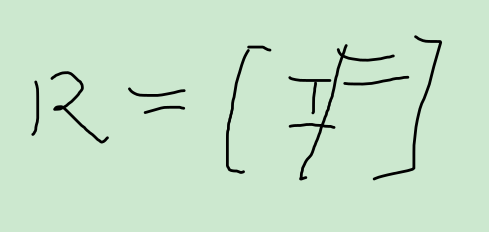
\includegraphics[width=0.3\textwidth]{figures/2021-09-17T190337+0800.png}
rather than
\(
R =
\begin{bmatrix}
	I & F
\end{bmatrix}
\)

There exists solutions. The number of equations \(>\) the number of unknowns.

\( \infty \) solutions.

We always have null space to deal with.

If we set all free variables to \(0\), the unique solution exists.

\subsection{\( r < m, r < n  \)}%
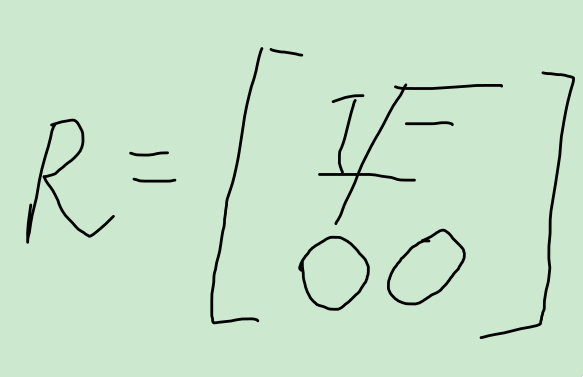
\includegraphics[width=0.3\textwidth]{figures/2021-09-17T191029+0800.png}

0 or \( \infty \) solutions

\begin{remark}
	The rank tells you everything about the number of solutions
\end{remark}

%%% vim: set ts=2 sts=2 sw=2 isk+=\: et cc=+1 formatoptions+=mM:
%
% 统计力学玻尔兹曼分布

\section{统计力学玻尔兹曼分布}
\subsubsection{体系的微观状态}
粒子的一个微观状态在\(\mu \)空间中对应一点,
一个体系的微观状态对应\(N\)个点,
粒子的微观状态随时间的变化对应一根线。
体系的微观状态随时间的变化对应\(N\)根线。
某个粒子的微观状态随时间变化的这根线不相交(与牛顿方程的单值性违背(保守力学体系))。

\subsection{相格}
引入相格。相格需
\begin{itemize}
  \item 足够大: 可含足够多代表点
  \item 足够小:一个相格内不同点的\(\{\vb{q}, \vb{p}\}\)看作近似相等
\end{itemize}
给相格进行编号,给粒子进行编号。
\begin{definition}[配容]
每个相格中既问有几点,又问哪几点的分配方式。
\end{definition}
同相格内部代表点交换,微观态不变,配容不变;
不同相格内部代表点交换,微观态变,配容变。

\subsection{体系的宏观状态}
每个相格中问有几点,不问哪几点。

一个宏观态对应多少微观态?
在不同相格交换的次数\({N!} / {\prod_l a_l!}\)。
\\ 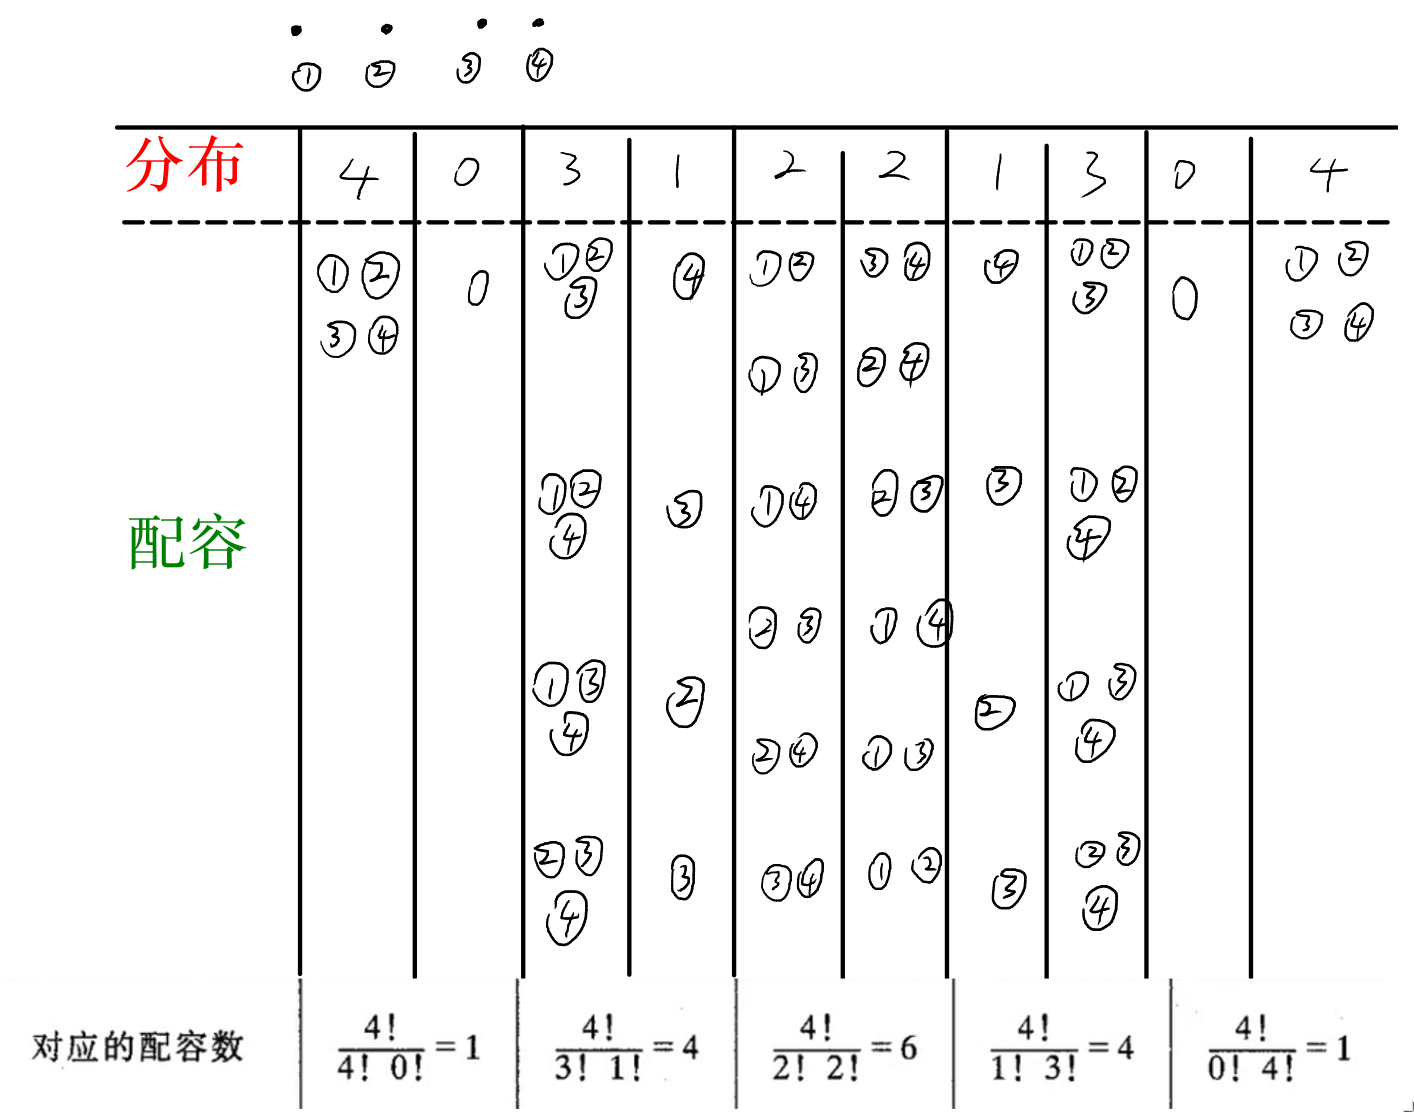
\includegraphics[width=0.8\textwidth]{figures/2022-09-07T220102+0800.png} \\

\subsection{体系的平衡态,最概然分布}
\begin{definition}[进入第\(l\)个相格的概率]
  \begin{equation}
    g_l = \frac{\Delta \omega_l}{\omega}
  \end{equation}
\end{definition}

基本假定:
\begin{enumerate}
  \item 先验\sn{不加约束条件}机率相等\sn{每个代表点进到相格的机率与相格的大小成比例}:\(g_i = g_j = \dots\)
  \item 平衡态是最可几\sn{出现机率最大}的宏观态
\end{enumerate}
\begin{margintable}
  \begin{description}
  \item[\(\Delta \omega_l\)]   第\(l\)个相格的体积  \\
  \item[\(g_l\)]   撒一颗豆子落到第\(l\)个相格的概率  \\
  \item[\(g_l^{a_l}\)]   撒N个豆子,有\(a_l\)颗落到第\(l\)个相格的概率
  \end{description}
\end{margintable}
\begin{marginfigure}
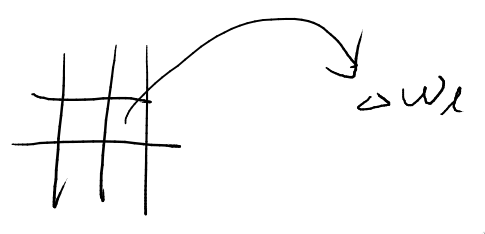
\includegraphics[width=\textwidth]{figures/2022-09-07T223529+0800.png} \\
\end{marginfigure}
对于某个宏观态,第$l$个相格有\(a_l\)个点,\(l \in [1, L]\),\(L\)为相格总数,则每个微观观态出现的概率都为
\begin{equation*}
  \underbrace{g_1 g_1 g_1\dots}_{a_1\text{个}}
  \underbrace{g_2 g_2 g_2\dots}_{a_2\text{个}}
  \underbrace{g_l g_l g_l\dots}_{a_l\text{个}}
  = \prod_l g_l^{a_l}
\end{equation*}
该宏观态有\({N!} / (\prod_l a_l !)\)个微观态,那么这个宏观态出现的概率为
\begin{equation}
  \begin{aligned}
  W 
  &=\underbrace{\left(\prod_l g_l^{a_l}+\prod_l g_l^{a_l}+\prod_l g_l^{a_l}+\dots\right)}_{\frac{N!}{\prod_l a_l!} \text{个微观态}} \\
  &= \frac{N!}{\prod_l a_l!} \prod_l g_l^{a_l}=
\frac{N!}{\prod_l a_l!}
\prod_l \left(\frac{\Delta \omega_l}{\omega}\right)^{a_l}\\
    &=
\left(\prod_l \frac{1}{\omega^{a_l}}\right)
\cdot
\left(\frac{N!}{\prod_l a_l!}
\prod_l {\Delta \omega_l}^{a_l}
\right) \\
    &=
\left(\frac{1}{\omega}\right)^{\sum_l a_l}
\cdot
\left(\frac{N!}{\prod_l a_l!}
\prod_l {\Delta \omega_l}^{a_l}
\right) \\
  \end{aligned}
\end{equation}
又因为每个微观态出现的先验机率相等
\begin{equation}
\prod_l g_l^{a_l}=\left(\frac{\Delta \omega_l}{\omega}\right)^{a_l}
=\left(\frac{\Delta \omega}{\omega}\right)^{a_l}
\end{equation}




%%% vim: set ts=2 sts=2 sw=2 isk+=\: et cc=+1 formatoptions+=mM:


% !TEX root = main.tex
% LaplaceTransform


\section{Laplace Transform}%
\subsection{由幂级数引入拉普拉斯变换}%
\begin{equation*}
	\sum_{n=1}^{\infty} a_n = A(x)
\end{equation*}

\begin{equation*}
	\sum_{n=1}^{\infty} a(n) = A(x)
\end{equation*}
If time continues
\begin{equation*}
	\int_{0}^{\infty} \red{a(t)} x^t \dd t = \blue{A(x)}  \qc \text{收敛条件:} 0<x<1
\end{equation*}
根据恒等式
\begin{gather*}
	x = e^{\ln x}\\
	x^t = e^{t \ln x}
\end{gather*}
\(-s = \ln x < 0 \implies s>0\)
\begin{remark}
	为什么要令 \(-s = \ln x\)?

	因为 \(\ln x\) 自然地限制了 \(x > 0\),只要再加一个条件\(\ln x < 0\) 就又限制了 \(x<1\)。
\end{remark}

\begin{equation*}
	\int_{0}^{\infty} \red{f(t)} e^{-st} \dd t = \blue{F(s)}  \qc \text{收敛条件:} s > 0
\end{equation*}

线性性质:
\begin{itemize}
	\item 加和:\(\La[f+g] = \La[f]+ \La[g]\)
	\item 数乘: \(\La[cf] = c \La[f]\)
\end{itemize}


% TODO
“基”相当于“自变量”,由于基改变了,线性变换称为变换

\begin{itemize}
	\item \(f(t)\) transform \(F(s)\)
	\item \(f(t) \) operator \(g(t)\)
\end{itemize}

\begin{equation*}
	\La[t^n] = \frac{n}{s} \La[t^{n-1}] = \frac{n!}{s^{n+1}}
\end{equation*}
	
\begin{equation*}
	\La[f'(t)] = s\La[f(t)] - f(0)
\end{equation*}
\begin{equation*}
	\La[f''(t)] = s\La[f'(t)] - f'(0)
\end{equation*}

Use Laplace transform to solve linear differential equations with constant coefficients.

Laplace Transform, exist?

Condition: \(f(t)\) doesn't grow so rapidly. ``exponential type''



%%% vim: set ts=2 sts=2 sw=2 isk+=\: et cc=+1 formatoptions+=mM:


% !TEX root = main.tex
% 有阻尼的受迫振子

\section{有阻尼的受迫振子}%
油,蜂蜜等浓的液体中,摩擦和速度成正比
\begin{equation*}
	f \propto v
\end{equation*}

\begin{equation*}
	f = -m \gamma \dot{x}
\end{equation*}

\begin{equation*}
	m \ddot{x} = F + f + F_{\text{回复}}
\end{equation*}

\begin{equation}
	m \ddot{x} + m \gamma \dot{x} + m \omega_0^2 x = F
	\label{eq:test}
\end{equation}

\begin{equation*}
	\hat{x} = \frac{\hat{F}}{m(\omega_0^2 - \omega^2 + i \omega)}
\end{equation*}
对式~\eqref{eq:test} 进行 \(\La^{-1}\)

\begin{equation*}
	\frac{\hat{x}}{\hat{F}} = \frac{1}{ m ( s^2 +\gamma s + \omega_0^2 ) }
\end{equation*}

令\( 2 \xi \omega_0 = \gamma \),仅仅为了求根的时候结果简洁
\begin{equation*}
	\frac{\hat{x}}{\hat{F}} = \frac{1}{ m ( s^2 + 2 \xi \omega_0 s + \omega_0^2 ) }
\end{equation*}

极点:
\begin{equation*}
	 s^2 + 2 \xi \omega_n s + \omega_n^2 = 0
\end{equation*}
根据求根公式
\begin{equation*}
	s = -\xi \omega_n \pm \sqrt{\xi^2 -1} \omega_n
\end{equation*}
当 \(0< \xi < 1\)
\begin{equation*}
	s = -\xi \omega_n \pm i \sqrt{1 - \xi^2 } \omega_n
\end{equation*}
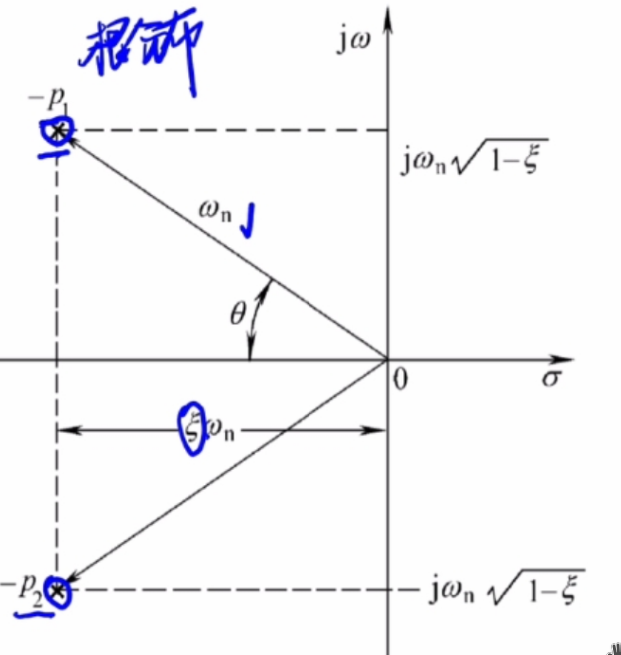
\includegraphics[width=0.4\textwidth]{figures/2021-09-23T004059+0800.png}
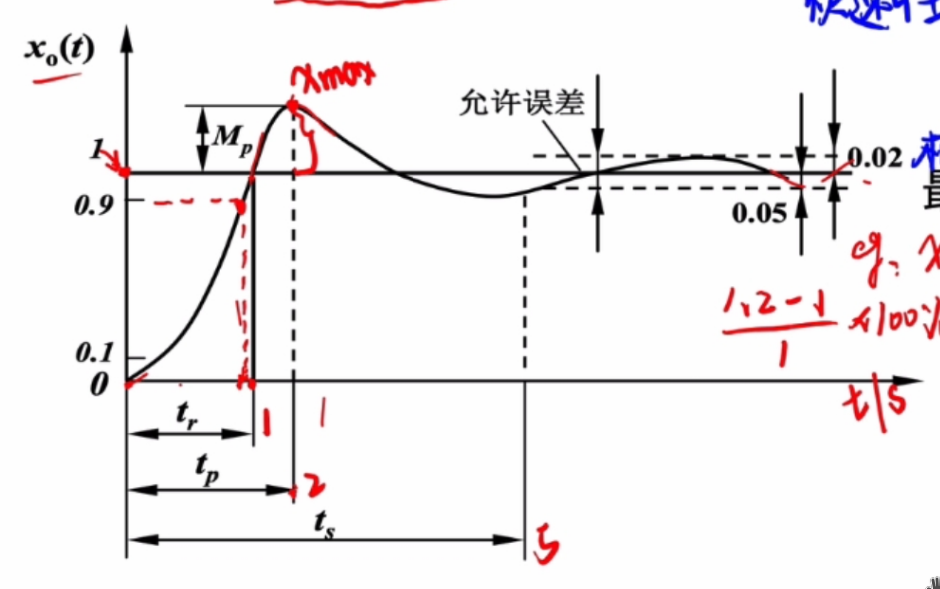
\includegraphics[width=0.5\textwidth]{figures/2021-09-23T004313+0800.png}

上升时间:
\begin{equation*}
	t_r = \frac{\pi - \theta}{ \omega_d } = \frac{\pi - \theta}{ \omega_n \sqrt{1 - \xi^2} }
\end{equation*}
\(\xi\)越大,上升时间越大。
这是显然的。
想象一个在油中的弹簧振子,先被压缩。
摩擦系数越大,达到平衡位置所花时间越长。

峰值(peak)时间:
\begin{equation}
	t_p = \frac{\pi}{ \omega_n \sqrt{1-\xi^2} }
\end{equation}
\(\xi\)越大,peak time 越大
调节时间:
\begin{equation*}
	t_s = \frac{3.5}{\xi \omega_n}
\end{equation*}

\(\xi\)越大,调节时间越小
这是显然的。
想象一个在油中的弹簧振子,先被压缩。
摩擦系数越大,更快静止。

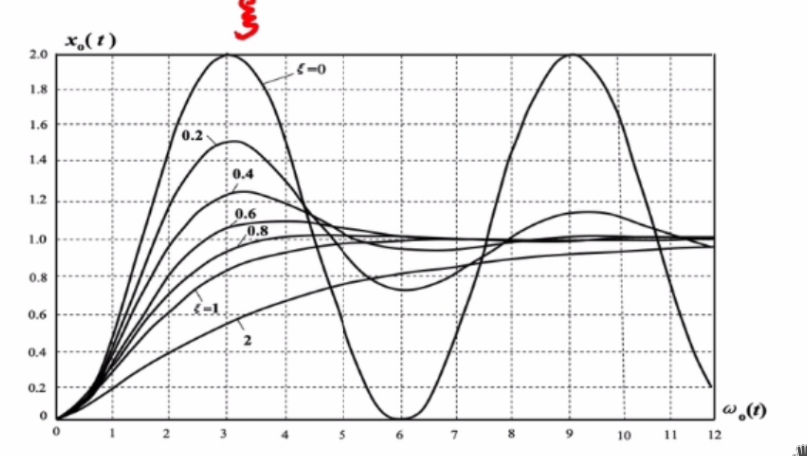
\includegraphics[width=0.5\textwidth]{figures/2021-09-23T011056+0800.png}





%%% vim: set ts=2 sts=2 sw=2 isk+=\: et cc=+1 formatoptions+=mM:



% 广义曲线坐标系拉普拉斯算子证明

\section{尝试证明}%
我们电动力学书上是直接给出梯度散度旋度拉普拉斯算符的,我对此一直很困惑

\begin{definition}[梯度]
	\begin{equation}
		\grad = \sum_i \frac{1}{\textcolor{red}{h_i}} \red{\pdv{x_i}} \vu{x}_i
		\label{eq:梯度}
	\end{equation}
\end{definition}

\begin{definition}[散度]
	\begin{equation}
		\label{eq:div}
		\div \vb{y}  = \frac{1}{\prod_i h_i} \sum_i \left[
			\pdv{x_i}( h'_i \red{y_i})
			\right]
		\qc
		h'_{i} = \prod_{j \neq i}  h_j
	\end{equation}
\end{definition}

我发现:\\
只要令 Eq.~\eqref{eq:div} 中 $\vb{y}$ 等于 $\grad$ \\
即:令$y_i=\frac{1}{\textcolor{red}{h_i}} \red{\pdv{x_i}} $ 塞进 Eq.~\eqref{eq:div}
\begin{definition}[拉普拉斯算子]

	\begin{equation}
		\div \grad \equiv \laplacian = \frac{1}{\prod_i h_i}
		\sum_i
		\left[
			\pdv{x_i}( \frac{h'_i}{\red{h_i}} \red{\pdv{x_i}})
			\right]
		\qc
		H_i = \frac{\prod_{j \neq i} h_j}{ h_i } =\frac{h'_i}{ h_i }
	\end{equation}
\end{definition}


\begin{definition}[旋度]
	\begin{equation}
		\curl \vb{y}  = \frac{1}{\prod_i h_i}
		\begin{vmatrix}
			\ldots & h_i  \vu{x}_i & \ldots \\
			\ldots & \pdv{x_i}     & \ldots \\
			\ldots & h_i y_i       & \ldots
		\end{vmatrix}
	\end{equation}
\end{definition}
先证明梯度,其他看起来大同小异。
直接列式子要写一大堆,用线性代数矩阵乘法来做要简洁些(满足结合律)。
\section{开始证明}%
\subsection{铺垫}%
\subsubsection{旋转矩阵}%
% 基矢变换
\begin{figure}[h]
	\centering
	\includesvg[width=0.3\linewidth]{figures/坐标系变换}
	\caption{直角坐标基矢变换为极坐标基矢}%
	% \label{fig:fig/坐标系变换}
\end{figure}

\begin{equation}
	\begin{aligned}
		% \label{eq:坐标变换方程}
		\vu{r}     & = \cos\phi \vu{i} + \sin\phi \vu{j}                                    \\
		\vu*{\phi} & = \cos(\phi+ \frac{\pi}{2}) \vu{i} + \sin(\phi + \frac{\pi}{2} )\vu{j}
	\end{aligned}
\end{equation}




写成矩阵形式

\begin{equation}
	% \label{Eq:矩阵形式的坐标变换}
	\mqty[ \vu{r} \\ \vu*{\phi}  ] =
	\mqty[
		\cos\phi & \sin\phi \\
		-\sin\phi &\cos\phi \\
	]
	\mqty[ \vu{i} \\ \vu{j} ]
\end{equation}

\begin{definition}[旋转矩阵\(\RR\)]
	\begin{equation}
		\RR =
		\mqty[
			\cos\phi & \sin\phi \\
			-\sin\phi &\cos\phi \\
		]
		\label{eq:旋转矩阵}
	\end{equation}
\end{definition}

\begin{remark}
	极坐标的旋转矩阵 好写,就是看图转下,\(\phi\) 多加 90度; 柱坐标也好写,在极坐标基础上多加一维;球坐标的旋转矩阵,就是在柱坐标基础上再转下,在柱坐标旋转矩阵基础上再乘一个矩阵
\end{remark}

通过观察法凑出基矢变换矩阵(对于球坐标也就是转两次的“旋转矩阵”)可以这样写:
\begin{equation}
    \label{eq:基矢变换矩阵}
  \begin{aligned}
    \RR &=
  \mqty[
  \frac{1}{h_1} \pdv{x}{r} &
  \frac{1}{h_1} \pdv{y}{r} &
  \frac{1}{h_1} \pdv{z}{r} \\
  \frac{1}{h_2} \pdv{x}{\theta} &
  \frac{1}{h_2} \pdv{y}{\theta} &
  \frac{1}{h_2} \pdv{z}{\theta} \\
  \frac{1}{h_3} \pdv{x}{\phi} &
  \frac{1}{h_3} \pdv{y}{\phi} &
  \frac{1}{h_3} \pdv{z}{\phi} \\] \\
        &=
        \mqty[
  \frac{1}{h_1}  &
  0  &
  0  \\
  0  &
  \frac{1}{h_2}  &
  0  \\
  0  &
  0  &
  \frac{1}{h_3}  \\
        ]
\mqty[
  \pdv{x}{r} &
  \pdv{y}{r} &
  \pdv{z}{r} \\
  \pdv{x}{\theta} &
  \pdv{y}{\theta} &
  \pdv{z}{\theta} \\
  \pdv{x}{\phi} &
  \pdv{y}{\phi} &
  \pdv{z}{\phi} \\] \\
                & = 
        \mqty[
  \frac{1}{h_1}  &
  0  &
  0  \\
  0  &
  \frac{1}{h_2}  &
  0  \\
  0  &
  0  &
  \frac{1}{h_3}  \\
        ]
        \JJ \tp
  \end{aligned}
\end{equation}


\vspace{1cm}
\subsubsection{雅可比矩阵}%
\begin{definition}[雅可比矩阵]
	\begin{equation}
		\label{eq:雅可比矩阵}
		\begin{aligned}
			\JJ             & =
			\left(
			\left(\pdv{\vb{x}}\right) \left(\vb{y}\right)\tp
			\right)\tp
			=
			\left(
			\begin{pmatrix}
					\pdv{r}      \\
					\pdv{\theta} \\
					\pdv{\phi}
				\end{pmatrix}
			\begin{pmatrix}
					x & y & z
				\end{pmatrix}
			\right)\tp                                                  \\
			                & =
			\pdv{(x,y,z)}{(r,\theta,\phi)}
			=
			\mqty[
			\pdv{x}{r}      & \pdv{x}{\theta}      & \pdv{x}{\phi}      \\
			\pdv{y}{r}      & \pdv{y}{\theta}      & \pdv{y}{\phi}      \\
			\pdv{z}{r}      & \pdv{z}{\theta}      & \pdv{z}{\phi}
			]
			=
			\mqty[
			\pdv{\vb{r}}{r} & \pdv{\vb{r}}{\theta} & \pdv{\vb{r}}{\phi}
			]
		\end{aligned}
	\end{equation}
\end{definition}

\vspace{1cm}
\subsubsection{拉梅系数}
\begin{equation}
  \label{eq:拉梅系数}
	h_i=\norm{\pdv{\vb{\vb{y}}}{x_i}} \qq{或写成}
	h_i=\norm{\pdv{\vb{\vb{r}}}{q_i}}
\end{equation}
\marginnote{看起来对雅可比矩阵的一列取模就是拉梅系数的值了?}
如表\ref{tab:lamei}所示。
\begin{table}[htpb]
	\centering
	\caption{拉梅系数.}
	\label{tab:lamei}
	\begin{tabular}{c|ccc}
		\toprule
		$(q_1,q_2,q_3)$ & 直角$(x,y,z) \tp$ & 柱 $(\rho, \phi, z) \tp$ & 球 $(r, \theta, \phi) \tp$ \\
		\midrule
		$h_1$           & $1$               & $1$                      & $1$                        \\
		$h_2$           & $1$               & $\rho$                   & $r$                        \\
		$h_3$           & $1$               & $1$                      & $r\sin\theta$              \\
		\bottomrule
	\end{tabular}
\end{table}
\subsection{证明的关键:旋转矩阵乘雅可比行列式}%
利用链式法则和式~\eqref{eq:雅可比矩阵} 可得
\begin{equation}
	\label{eq:链式法则}
	\mqty[
		\pdv{u}{r} \\ \pdv{u}{\phi}
		\\ \pdv{u}{\theta}
	]
	=
	\mqty[
		\pdv{x}{r} & \pdv{x}{\phi} & \pdv{x}{\theta} \\
		\pdv{y}{r} & \pdv{y}{\phi} & \pdv{y}{\theta} \\
		\pdv{z}{r} & \pdv{z}{\phi} & \pdv{z}{\theta} \\
	] \tp
	\mqty[
		\pdv{u}{x} \\ \pdv{u}{y}
		\\ \pdv{u}{z}
	]
	= \JJ \tp
	\mqty[
		\pdv{u}{x} \\ \pdv{u}{y}
		\\ \pdv{u}{z}
	]  \\
\end{equation}
\begin{equation*}
	\mqty[
		\pdv{u}{x} \\ \pdv{u}{y}
		\\ \pdv{u}{z}
	]
	=
	\mqty[
		\pdv{r}{x} & \pdv{\phi}{x} & \pdv{\theta}{x} \\
		\pdv{r}{y} & \pdv{\phi}{y} & \pdv{\theta}{y} \\
		\pdv{r}{z} & \pdv{\phi}{z} & \pdv{\theta}{z} \\
	]
	\mqty[
		\pdv{u}{r} \\ \pdv{u}{\phi}
		\\ \pdv{u}{\theta}
	]
	= (\JJ  \tp)^{-1}
	\mqty[
		\pdv{u}{r} \\ \pdv{u}{\phi}
		\\ \pdv{u}{\theta}
	]
\end{equation*}
\begin{equation*}
	\mqty[
		\pdv{u}{x} \\ \pdv{u}{y}
		\\ \pdv{u}{z}
	] \tp
	=
	\mqty[
		\pdv{u}{r} \\ \pdv{u}{\phi}
		\\ \pdv{u}{\theta}
	] \tp
	\mqty[
		\pdv{r}{x} & \pdv{\phi}{x} & \pdv{\theta}{x} \\
		\pdv{r}{y} & \pdv{\phi}{y} & \pdv{\theta}{y} \\
		\pdv{r}{z} & \pdv{\phi}{z} & \pdv{\theta}{z} \\
	] \tp
	= ((\JJ  \tp)^{-1})\tp
	\mqty[
		\pdv{u}{r} \\ \pdv{u}{\phi}
		\\ \pdv{u}{\theta}
	]
	= \JJ^{-1}
	\mqty[
		\pdv{u}{r} \\ \pdv{u}{\phi}
		\\ \pdv{u}{\theta}
	]
\end{equation*}
直角坐标的梯度可以这样写:
\begin{equation}
	\label{eq:直角坐标梯度}
	\begin{aligned}
		\grad u    & =
		\mqty[
		\pdv{u}{x} & \pdv{u}{y}
		           & \pdv{u}{y}
		]
		\mqty[
		\vu{i}                  \\
		\vu{j}                  \\
		\vu{k}                  \\
		]                       \\
	\end{aligned}
\end{equation}
把式~\eqref{eq:旋转矩阵}和式~\eqref{eq:链式法则} 带入式~\eqref{eq:直角坐标梯度},并把式~\eqref{eq:梯度}写成矩阵形式:
\begin{equation}
	\begin{aligned}
		\grad u       & =
		\mqty[
		\pdv{u}{r}    & \pdv{u}{\phi}
		              & \pdv{u}{\theta}
		]
		\red{\JJ^{-1} \RR \tp
		}\mqty[
		\vu{r}                                          \\
		\vu{\phi}                                       \\
		\vu{\theta}                                     \\
		]                                               \\
		              & =
		\mqty[
		\pdv{u}{r}    & \pdv{u}{\phi}
		              & \pdv{u}{\theta}
		]
		\red{\mqty[
		\frac{1}{h_1} & 0               & 0             \\
		0             & \frac{1}{h_2}   & 0             \\
		0             & 0               & \frac{1}{h_3}
			]}
		\mqty[
		\vu{r}                                          \\
		\vu{\phi}                                       \\
		\vu{\theta}                                     \\
		]                                               \\
	\end{aligned}
\end{equation}
\marginnote{我猜想红色的式子是普遍相等的}

\begin{equation*}
	\JJ^{-1} \RR \tp
	=
	\mqty[
		\frac{1}{h_1} &0&0 \\
		0&\frac{1}{h_2}&0 \\
		0&0&\frac{1}{h_3}
	]
\end{equation*}

\begin{equation*}
	(\JJ^{-1} \RR \tp)^{-1}
	=
	\RR \JJ
	=
	\mqty[
		h_1 &0&0 \\
		0&h_2&0 \\
		0&0& h_3
	]
\end{equation*}
将式~\eqref{eq:基矢变换矩阵} 带入:
\begin{equation*}
  \begin{aligned}
    \RR \JJ &= 
        \mqty[
  \frac{1}{h_1}  &
  0  &
  0  \\
  0  &
  \frac{1}{h_2}  &
  0  \\
  0  &
  0  &
  \frac{1}{h_3}  \\
        ]
\mqty[
  \pdv{x}{r} &
  \pdv{y}{r} &
  \pdv{z}{r} \\
  \pdv{x}{\theta} &
  \pdv{y}{\theta} &
  \pdv{z}{\theta} \\
  \pdv{x}{\phi} &
  \pdv{y}{\phi} &
  \pdv{z}{\phi} \\]
			\mqty[
			\pdv{x}{r}      & \pdv{x}{\theta}      & \pdv{x}{\phi}      \\
			\pdv{y}{r}      & \pdv{y}{\theta}      & \pdv{y}{\phi}      \\
			\pdv{z}{r}      & \pdv{z}{\theta}      & \pdv{z}{\phi}
			] \\
                      &=
        \mqty[
  \frac{1}{h_1}  &
  0  &
  0  \\
  0  &
  \frac{1}{h_2}  &
  0  \\
  0  &
  0  &
  \frac{1}{h_3}  \\
        ] 
        \JJ \tp \JJ
  \end{aligned}
\end{equation*}

也就是证明:
\begin{equation}
  \label{eq:拉梅系数平方}
        \JJ \tp \JJ
        =
        \mqty[
        h_1^2 & 0 & 0 \\
        0 & h_2^2 & 0 \\
        0 & 0 & h_3^2 \\
        ]
\end{equation}
由拉梅系数定义式~\eqref{eq:拉梅系数} 知,只需要证明雅可比矩阵正交

% \inputminted[linenos,numbersep=5pt,frame=lines,framesep=2mm]{wolfram}{./j.mma}
\code{wolfram}{./j.mma}
用 Mathematica 验证发现对于极坐标,柱坐标,球坐标,雅可比矩阵都满足式~\eqref{eq:拉梅系数平方} 。
% \(\RR \JJ =\text{\mintinline{matlab}{diag([h1,h2,h3])}}\)
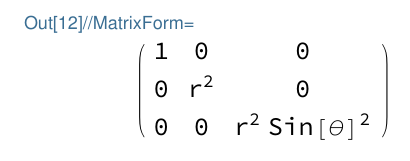
\includegraphics[width=0.5\textwidth]{figures/2021-10-13T133210+0800.png} 


\subsection{没证明出来的地方}%
\begin{itemize}
  \item 如果给出任意变换,如何写出基矢变换矩阵~\eqref{eq:基矢变换矩阵} 
  \item 雅可比矩阵正交
\end{itemize}


%%% vim: set ts=2 sts=2 sw=2 isk+=\: et cc=+1 formatoptions+=mM:


% !TEX root = main.tex
% 加权平均

\section{加权平均}%

一维:\(x\)轴被无限细分成小块,第\(i\)块为\(\Delta x_i\),这第\(i\)小块内有\(\Delta m_i\)落入其中
\begin{tabular}{ccc}
	\(\Delta x_1\) &   对应 & \(\Delta m_1\) \\
	\(\Delta x_2\) &   对应 & \(\Delta m_2\) \\
	\(\Delta x_3\) &   对应 & \(\Delta m_3\) \\
	\(\Delta x_4\) &   对应 & \(\Delta m_4\) \\
	…… & 对应 & …… \\
	\(\Delta x_n\) &   对应 & \(\Delta m_n\)
\end{tabular}

总质量是对所有质量块的求和:
\begin{equation*}
	m = \sum_i \Delta  m_i
\end{equation*}
质心
\begin{equation*}
	x_c =
	\frac{ \sum_i \Delta x_i \Delta m_i }{\sum_i \Delta m_i}
\end{equation*}
定义 \(\rho(x)\) 为线密度
, 在全空间积分
\begin{align*}
	m &= \int \dd m \\
	x_c  &= \frac{1}{m} \int x \dd m \\
	&= \frac{1}{m} \int_{-\infty}^{\infty} x \dv{m}{x} \dd x \\
	&= \frac{1}{m} \int_{-\infty}^{\infty} x \rho(x) \dd x \\
\end{align*}


平均时间
\begin{equation*}
	\tau =
	\frac{ \sum_i \Delta n_i \Delta t_i }{\sum_i \Delta n_i}
\end{equation*}
\begin{align*}
	- \dd n = n \lambda \dd t \\
	n = n_0 e^{-\lambda t}
\end{align*}
\begin{align*}
	\tau &=
	\frac{1}{n_0} \int^0_{n_0} t \dd n \\
			 &=
	\frac{1}{n_0} \int_0^{n_0} t \red{( - \dd n )} \\
			 &=
	\frac{1}{n_0} \int_0^{\infty} t \red{(n \lambda \dd t)} \\
			 &=
	\frac{1}{n_0} \int_0^{\infty} t \red{(n_0 e^{-\lambda t} \lambda \dd t)} \\
\end{align*}

平均能量

有\(a_l\) 个粒子能量为 \(\varepsilon_l\)
\begin{tabular}{ccc}
	\( a_1\) &   个粒子能量为 & \( \varepsilon_1\) \\
	\( a_2\) &   个粒子能量为 & \( \varepsilon_2\) \\
	\( a_3\) &   个粒子能量为 & \( \varepsilon_3\) \\
	\( a_4\) &   个粒子能量为 & \( \varepsilon_4\) \\
	…… & 个粒子能量为& …… \\
	\( a_n\) &   个粒子能量为 & \( \varepsilon_n\)
\end{tabular}
\begin{equation}
	\label{eq:planck_ave_energy}
	\overline{\varepsilon} = \frac{\sum_l a_l \varepsilon_l}{\sum_l a_l} = - \pdv{\ln Z}{\beta} = \frac{h \nu}{\exp(\frac{h\nu}{kT}) - 1}
\end{equation}





%%% vim: set ts=2 sts=2 sw=2 isk+=\: et cc=+1 formatoptions+=mM:


% !TEX root = main.tex
% 利用平方差公式降阶

\section{利用平方差公式降阶}%

\subsection{波动方程,达朗贝尔行波法}%

\begin{equation*}
	\da \psi = 0
\end{equation*}
\begin{equation*}
	\left(	\pdv[2]{x} + \pdv[2]{ict} \right)
	\psi = 0
\end{equation*}
\begin{equation*}
	\left(	\pdv[2]{x} - \pdv[2]{ct} \right)
	\psi = 0
\end{equation*}
\begin{equation*}
\pdv{x} \to \hat{x}
\qquad
\pdv{t} \to \hat{t}
\end{equation*}

\begin{equation*}
	\left(\hat{x}+\hat{t}\right) 
	\left(\hat{x}-\hat{t}\right) 
	\psi = 0
\end{equation*}
\begin{equation*}
	\pdv{\xi} \pdv{\eta} \psi = 0
\end{equation*}


\begin{equation*}
	\vb{v} = \matr{A} \vb{u}
\end{equation*}
\(\matr{A}\) 是常矩阵
\begin{equation*}
	\pdv{\vb{v}} = (\matr{A}^{-1})\tp \pdv{\vb{u}}
\end{equation*}
\sn{自己证}

\subsection{一维谐振子}%
\begin{equation*}
	\begin{aligned}
		\Ham &=  \hat{U} + \hat{T} \\
				 &= \frac{1}{2} m \omega^2 x^2 - \frac{\hbar^2}{2m} \pdv[2]{x} \\
				 &= \frac{1}{2m} ( m^2 \omega^2 x^2  - \hbar^2\pdv[2]{x}) \\
				 &= \frac{1}{2m} 
				 ( m \omega x  - \hbar\pdv{x})
				 ( m \omega x  + \hbar\pdv{x}) \\
				 &= \frac{1}{2m} 
				 a_+ \vdot a_-
	\end{aligned}
\end{equation*}
\subsection{克莱因高登方程和狄拉克方程}%



%%% vim: set ts=2 sts=2 sw=2 isk+=\: et cc=+1 formatoptions+=mM:


% !TEX root = main.tex
% 勒让德多项式

\section{勒让德多项式}%
\begin{equation*}
	\begin{aligned}
		P_l(x) &= \frac{1}{2^l} \sum_{m=0}^{[\frac{l}{2}]}
	(-1)^m C_l^m C_{2l - 2m}^{l} x^{l - 2m}\\
&= \frac{1}{2^l} \sum_{m=0}^{[\frac{l}{2}]}
	(-1)^m \frac{(2l - 2m)!}{m! (l-m)! (l-2m)!} x^{l-2m}
	\end{aligned}
\end{equation*}
其中\([\ ]\)代表向下取整
\begin{equation*}
	\left[\frac{l}{2}\right] = 
	\begin{cases}
		\frac{l}{2} & \qq{\(l\) is even } \\
		\frac{l-1}{2} & \qq{\(l\) is odd }
	\end{cases}
\end{equation*}

\begin{align*}
	P_0 = 1 \\
	P_1 = x \\
	P_2 = \frac{1}{2}(3x^2 - 1) \\
	P_3 = \frac{1}{2}(5x^3 - 3x)
\end{align*}





%%% vim: set ts=2 sts=2 sw=2 isk+=\: et cc=+1 formatoptions+=mM:
%
% !TEX root = main.tex
% 静电场唯一性定理

\section{静电场唯一性定理}%
\subsection{第一唯一性定理}%
边界条件给定,假设
\begin{equation*}
	\laplacian \phi = - \frac{\rho}{\epsilon_0}
\end{equation*}
有两个解\(\phi_1, \phi_2\),现证明\(\phi_1 = \phi_2\),设\(\phi_3 = \phi_2 - \phi_1\)。

内部:
\begin{equation*}
	\laplacian \phi_1 = - \frac{\rho}{\epsilon_0}
\end{equation*}
\begin{equation*}
	\laplacian \phi_2 = - \frac{\rho}{\epsilon_0}
\end{equation*}
\begin{equation*}
	\laplacian \phi_3 = 0
\end{equation*}
边界上:
\begin{equation}
\phi_3 = \phi_2 - \phi_1 = 0
\end{equation}
\begin{equation*}
	\pdv{\phi_3}{r}
	=
	\pdv{\phi_2}{r}
	-
	\pdv{\phi_1}{r}
	=0
\end{equation*}

利用矢量恒等式:
\begin{equation*}
	\div(\phi \grad \phi) 
	= 
	(\grad \phi) \vdot (\grad \phi) 
	+
	\phi \laplacian \phi
	= 
	(\grad \phi)^2
	+
	\phi \laplacian \phi
\end{equation*}

再利用散度定理:
\begin{equation*}
	\oint \phi_3 \grad \phi_3 \vdot \dd \vb{S} 
	= 
	\int
	\left( 
	(\grad \phi_3)^2
	+
	\phi_3 \laplacian \phi_3\right)
	\dd V
\end{equation*}

由于\(\laplacian \phi_3=0\),所以
\begin{equation*}
	\oint \phi_3 \grad \phi_3 \vdot \dd \vb{S} 
	= 
	\int
	\left(\grad \phi_3\right)^2
	\dd V
\end{equation*}
由于边界处\(\phi_3 = 0\)且\(\grad \phi_3 = 0\)
\begin{equation*}
0 =
	\int
	\left(\grad \phi_3\right)^2
	\dd V
\end{equation*}
由于\(	\left(\grad \phi_3\right)^2 \geq 0\),所以
\begin{equation*}
	\grad \phi_3 = 0
\end{equation*}
所以\(\phi_3\)为常数,又由于\(\phi_3\)在边界处为零,若\(\phi_3\)连续
\begin{equation*}
	\phi_3 = 0
\end{equation*}
即
\begin{equation*}
 \phi_2 = \phi_1
\end{equation*}

\subsection{第二唯一性定理}%

\begin{equation*}
	\div(\grad \phi_1 )= \frac{\rho}{\epsilon}
\end{equation*}
\begin{equation*}
	\div(\grad \phi_2 )= \frac{\rho}{\epsilon}
\end{equation*}
\begin{equation*}
	\div\left(\grad (\phi_2 - \phi_1) \right)=0
\end{equation*}

导体的边界上:
\begin{equation*}
	\oint (\grad \phi_1 ) \vdot \dd \vb{S}= \frac{Q}{\epsilon}
\end{equation*}
\begin{equation*}
	\oint (\grad \phi_2 ) \vdot \dd \vb{S}= \frac{Q}{\epsilon}
\end{equation*}
\begin{equation}
	\oint (\grad \phi_3 ) \vdot \dd \vb{S}=0
	\label{eq:ophi3}
\end{equation}

矢量恒等式:
\begin{equation*}
	\div(\phi \grad \phi) 
	= 
	(\grad \phi) \vdot (\grad \phi) 
	+
	\phi \laplacian \phi
	= 
	(\grad \phi)^2
	+
	\phi \laplacian \phi
\end{equation*}

再利用散度定理:
\begin{equation*}
	\oint \phi_3 \grad \phi_3 \vdot \dd \vb{S} 
	= 
	\int
	\left( 
	(\grad \phi_3)^2
	+
	\phi_3 \laplacian \phi_3\right)
	\dd V
\end{equation*}

由于\(\laplacian \phi_3=0\),所以
\begin{equation*}
	\oint \phi_3 \grad \phi_3 \vdot \dd \vb{S} 
	= 
	\int
	\left(\grad \phi_3\right)^2
	\dd V
\end{equation*}
由于导体是等势体,\(\phi_3\)在边界处是个常数
\begin{equation*}
\phi_3 	\oint \grad \phi_3 \vdot \dd \vb{S} 
	= 
	\int
	\left(\grad \phi_3\right)^2
	\dd V
\end{equation*}
Eq.~\eqref{eq:ophi3} 
\begin{equation*}
	0
	= 
	\int
	\left(\grad \phi_3\right)^2
	\dd V
\end{equation*}
由于\(	\left(\grad \phi_3\right)^2 \geq 0\),所以
\begin{equation*}
	\grad \phi_3 = 0
\end{equation*}




%%% vim: set ts=2 sts=2 sw=2 isk+=\: et cc=+1 formatoptions+=mM:


% Einstein求和约定

\section{Einstein求和约定}%
\begin{equation*}
	\begin{aligned}
		& \varepsilon_{ijk}(\partial_i \partial_j \phi)(\partial_k) \\
		&= 
		\frac{1}{2}\varepsilon_{ijk}(\partial_i \partial_j \phi)(\partial_k)
		+
		\frac{1}{2}\varepsilon_{ijk}(\partial_i \partial_j \phi)(\partial_k) \\
		&= 
		\frac{1}{2}\varepsilon_{ijk}(\partial_i \partial_j \phi)(\partial_k) 
		+
		\frac{1}{2}\varepsilon_{jik}(\partial_j \partial_i \phi)(\partial_k) \\
		&= 
		\frac{1}{2}\varepsilon_{ijk}(\partial_i \partial_j \phi)(\partial_k) 
		+
		\frac{1}{2}\varepsilon_{jik}(\partial_i \partial_j \phi)(\partial_k) \\
		&= 
		\frac{1}{2}\varepsilon_{ijk}(\partial_i \partial_j \phi)(\partial_k) 
		-
		\frac{1}{2}\varepsilon_{ijk}(\partial_i \partial_j \phi)(\partial_k)
	\end{aligned}
	\left( kjkj \right)
\end{equation*}





%%% vim: set ts=2 sts=2 sw=2 isk+=\: et cc=+1 formatoptions+=mM:

% !TEX root = main.tex
% 泰勒展开
\section{泰勒展开}
乘积顺序不能换,但直积和点积,结合律还是能用的(和点积与叉积不同,因为矢量叉乘得到矢量,矢量点积得到标量)
\begin{equation*}
	\int \dd V \div(\vb{j}\vb{x}) 
	= \oint \dd \vb{S} \vdot (\vb{j}\vb{x}) 
	= \oint (\dd \vb{S} \vdot \vb{j})\vb{x} 
\end{equation*}
\(- \vb{x'}\) 为小量
\begin{equation*}
	\begin{aligned}
	\frac{1}{ \abs{\vb{x} - \vb{x'}} }
	&= \frac{1}{0!} \frac{1}{\abs{\vb{x}}}
	+ \frac{1}{1!} (\vb{-x'}) \vdot \grad \frac{1}{\abs{\vb{x}}}
	+ \frac{1}{2!} (\vb{-x'}) (\vb{-x'}) : \grad\grad \frac{1}{\abs{\vb{x}}} \\
	&= \frac{1}{0!} \frac{1}{\abs{\vb{x}}}
	- \frac{1}{1!} \vb{x'} \vdot  \grad \frac{1}{\abs{\vb{x}}}
	+ \frac{1}{2!} \vb{x'}\vb{x'} : \grad\grad \frac{1}{\abs{\vb{x}}}
	\end{aligned}
\end{equation*}
\begin{equation*}
	\Delta \phi = \grad \phi \vdot \Delta \vb{x}
\end{equation*}
\begin{equation*}
	 \phi(\vb{x} + \Delta \vb{x}) - \phi(\vb{x})  = \grad \phi \vdot \Delta \vb{x}
\end{equation*}
\begin{equation*}
	 \phi(\vb{x} + \Delta \vb{x}) = \phi(\vb{x})  + \grad \phi \vdot \Delta \vb{x}
\end{equation*}
\begin{equation*}
	 \phi(\vb{x} + \Delta \vb{x}) = \phi(\vb{x})  +  \Delta \vb{x}\vdot \grad \phi
\end{equation*}
\begin{equation*}
	 \phi(\vb{x} + \Delta \vb{x}) = \frac{1}{0!} \phi(\vb{x})  + \frac{1}{1!} \Delta \vb{x}\vdot \grad \phi
\end{equation*}
\begin{equation*}
	 \phi(\vb{x} + \Delta \vb{x}) = \frac{1}{0!} \phi(\vb{x})  +
	 \frac{1}{1!} \Delta \vb{x}\vdot \grad \phi(\vb{x})
	 + \frac{1}{2!} \Delta \vb{x} \Delta \vb{x} : \grad \grad \phi(\vb{x}) 
\end{equation*}
类似地,矢量的泰勒展开
\begin{equation*}
	 \vb{B}(\vb{x} + \Delta \vb{x}) = \frac{1}{0!} \vb{B}(\vb{x})  +
	 \frac{1}{1!} \eqnmarkbox[Plum]{DirectionalDerivative}{\Delta \vb{x}\vdot \grad} \vb{B}(\vb{x})
	 + \frac{1}{2!} \Delta \vb{x} \Delta \vb{x} : \grad \grad \vb{B}(\vb{x}) 
\end{equation*}
\annotate[yshift=1em]{above}{DirectionalDerivative}{\# 方向导数}


%%% vim: set ts=2 sts=2 sw=2 isk+=\: et cc=+1 formatoptions+=mM:

% !TEX root = main.tex
% 电偶极子

\section{电偶极子}%
正负点电荷起初都在原点,
对于正电荷,场点向下移动,
等效于源点向上移动\(-\Delta \vb{r} = \Delta \vb{r}'\)
\begin{equation*}
	\Delta \phi_+=\phi'_+ - \phi_+ =
	\grad \phi_+ \vdot (-\Delta \vb{r})
	=\grad \phi_+ \vdot \Delta \vb{r}'
\end{equation*}
\begin{equation*}
	\phi'_+ = \phi_+ +
	\grad \phi_+ \vdot (-\Delta \vb{r})
\end{equation*}
对于负电荷,场点向上移动,等效于源点向下移动
\(\Delta \vb{r} = - \Delta \vb{r}'\)
\begin{equation*}
	\phi'_- =
	\phi_- + \grad \phi_- \vdot \Delta \vb{r}
\end{equation*}
向上移动的正点电荷与向下移动的负点电荷的线性叠加
\begin{equation*}
	\phi_+' + \phi_-' = 
	\grad \phi_+ \vdot 2 \Delta \vb{r}'
	=
	\grad \phi_+ \vdot \vb{d}
	=
	q \vb{d}  \vdot \grad \frac{1}{r}
\end{equation*}
记 \(q\vb{d}\) 为 \(\vb{p}\),电偶极子的位置就是正负电荷的中间,原点处电偶极子的势函数:
\begin{equation*}
	\phi = \phi_+' + \phi_-' = 
	-\vb{p} \vdot \grad \frac{1}{r}
\end{equation*}
若电偶极子不在原点:
\begin{equation*}
	\phi =
	- \vb{p} \vdot \grad \frac{1}{R}
\end{equation*}
注意到\(\grad \frac{1}{R} = - \frac{\vu{R}}{R^2}\)
\begin{equation*}
	\phi =
	 \frac{\vb{p} \vdot \vu{R}}{R^2}
\end{equation*}
补全系数
\begin{equation}
	\phi =
  \frac{1}{4 \pi \epsilon_0}
	 \frac{\vb{p} \vdot \vu{R}}{R^2}
\end{equation}
电偶极子电场:
\begin{equation}
  \vb{E} = \grad \phi= \frac{1}{4 \pi \epsilon_0} \left( \frac{\vb{p}}{R^3} - \frac{3\vb{p \vdot \vb{R}}}{R^5} \vb{R}\right)
\end{equation}
磁偶极子磁场
\begin{equation}
  \vb{B} = \curl \vb{A}= \frac{\mu_0}{4 \pi} \left( \frac{\vb{m}}{R^3} - \frac{3\vb{m \vdot \vb{R}}}{R^5} \vb{R}\right) 
\end{equation}
多个电偶极子势的线性叠加
\begin{equation*}
	\begin{aligned}
	  \sum_i \phi_i(\vb{r}) &=
	\sum_i {\vb{p}_i \vdot }{\grad \frac{1}{R_i}} \\
  &=
	 \int \dd \tau' \vb{P}  \vdot \grad \frac{1}{R} \\
  &=
	 \int \dd \tau'\div (  \frac{\vb{P}}{R}) -
	 \int \dd \tau'\left(\div \vb{P} \right)   \frac{1}{R} \\
  &=
	 \oint \dd \vb{S}' \vdot\vb{P} \frac{1}{R} -
	 \int \dd \tau'\left(\div \vb{P} \right)   \frac{1}{R} \\
  &=
	 \oint \dd S'  \frac{\sigma_b}{R} +
	 \int \dd \tau'  \frac{\rho_b}{R} \\
	\end{aligned}
\end{equation*}


%%% vim: set ts=2 sts=2 sw=2 isk+=\: et cc=+1 formatoptions+=mM:

% 等离子体基础第二次作业

\section{等离子体基础第二次作业}

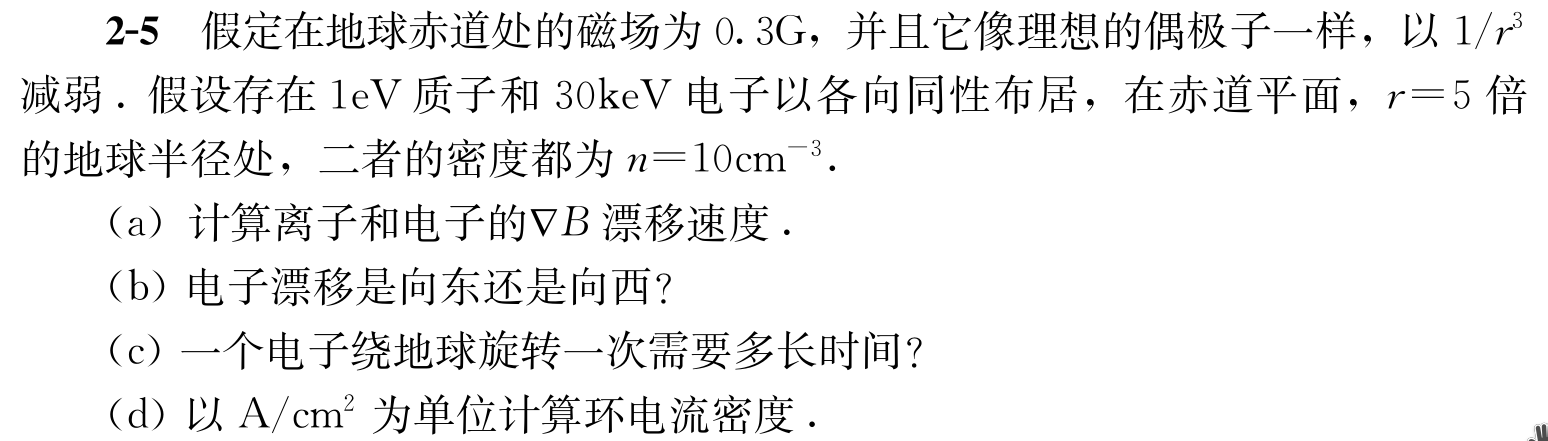
\includegraphics[width=0.9\textwidth]{figures/2022-09-30T114621+0800.png}

\subsection{Solution to 2-5}
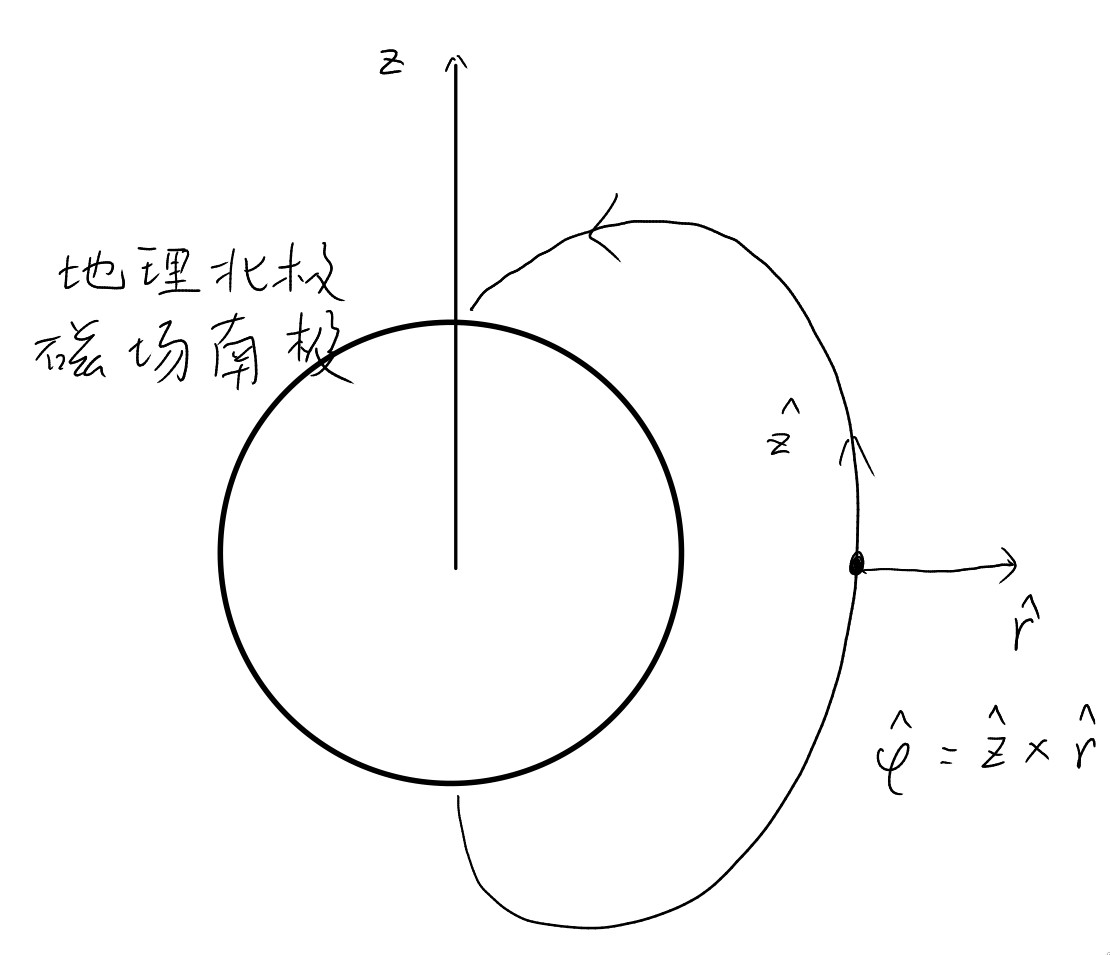
\includegraphics[width=0.5\textwidth]{figures/2022-09-30T114803+0800.png} \\

\noindent \textbf{(a)} 
如图所示,粒子垂直于磁场方向的速度\(v_{\perp}\)有两个自由度构成,
\begin{equation}
  \frac{1}{2} m v_\perp^2 = \frac{i}{2}kT = k_BT
\end{equation}
将质子的漂移速度\(\vb{v}_{\grad B}\)记为\(\vb{v}_p\),
将电子的漂移速度\(\vb{v}_{\grad B}\)记为\(\vb{v}_e\),
根据书本的式(2-24)
\begin{equation}
  \vb{v}_{\grad B} = \pm \frac{1}{2} v_{\perp} r_L \frac{\vb{B} \cross \grad B}{B^2}
  \label{eq:v}
\end{equation}
其中 Larmor radius 为
\begin{equation}
  r_L = \frac{m v_\perp c}{\abs{q} B_G}
\end{equation}
设地球赤道处的磁场\(B_0 = B(r_0) = 0.3 \si{G}\),则磁感应强度方向沿着\(\vu{z}\)方向,
表达式为
\begin{equation}
  \vb{B} = \frac{B_0 r_0^3}{r^3}  \vu{z}= \frac{K}{r^3} \vu{z}
\end{equation}
磁场大小梯度
\begin{equation}
  \grad B = \pdv{B}{r} \vu{r} = -\frac{3 K}{r^4} \vu{r}
\end{equation}
带入式~\eqref{eq:v} 可得电子漂移速度
\begin{equation}
  \begin{aligned}
    \vb{v}_e &= - \eval{\frac{1}{2} v_{\perp} r_L \frac{\vb{B} \cross \grad B}{B}}_{r=5r_0}\\
             &= \eval{\frac{3}{2} \frac{m_e v_\perp^2 cr^2}{q K}  \vu{\phi}}_{r=5 r_0} \\
             &= \eval{ \frac{3 k_B T_e cr^2}{q K}  \vu{\phi}}_{r=5 r_0} \\
             &= 25 \times \frac{3 k_B T_e c}{q B_0 r_0}  \vu{\phi} \\
             &= \SI{1.17e8}{cm / s}
  \end{aligned}
\end{equation}
质子漂移速度
\begin{equation}
  \begin{aligned}
    \vb{v}_p &= \eval{\frac{1}{2} v_{\perp} r_L \frac{\vb{B} \cross \grad B}{B}}_{r=5r_0}\\
             &= -\eval{\frac{3}{2} \frac{m_p v_\perp^2 c r^2 }{q K} \vu{\phi}}_{r=5 r_0} \\
             &= -\eval{\frac{3 k_B T_p c r^2 }{q K} \vu{\phi}}_{r=5 r_0} \\
             &= -25\times \frac{3 k_B T_p c }{q B_0 r_0} \vu{\phi} \\
             &= \SI{3906.25}{cm / s}
  \end{aligned}
\end{equation}

\noindent \textbf{(b)} 电子漂移向东。

\noindent \textbf{(c)}
\begin{equation}
    \Delta \tau = 
  \eval{\frac{2 \pi r}{v_e}}_{r=5 r_0} = 343.15s
\end{equation}

\noindent \textbf{(d)}
\begin{equation}
    \vb{J} = \vb{J}_p + \vb{J}_e = ne(\vb{v}_p - \vb{v}_e) = \SI{1.87e-10}{A/cm^2}
\end{equation}


%%% vim: set ts=2 sts=2 sw=2 isk+=\: et cc=+1 formatoptions+=mM:

\end{document}
